\newcommand{\FigICEDUSTOverview}{
\begin{figure}[t]
\centering
%\fbox{
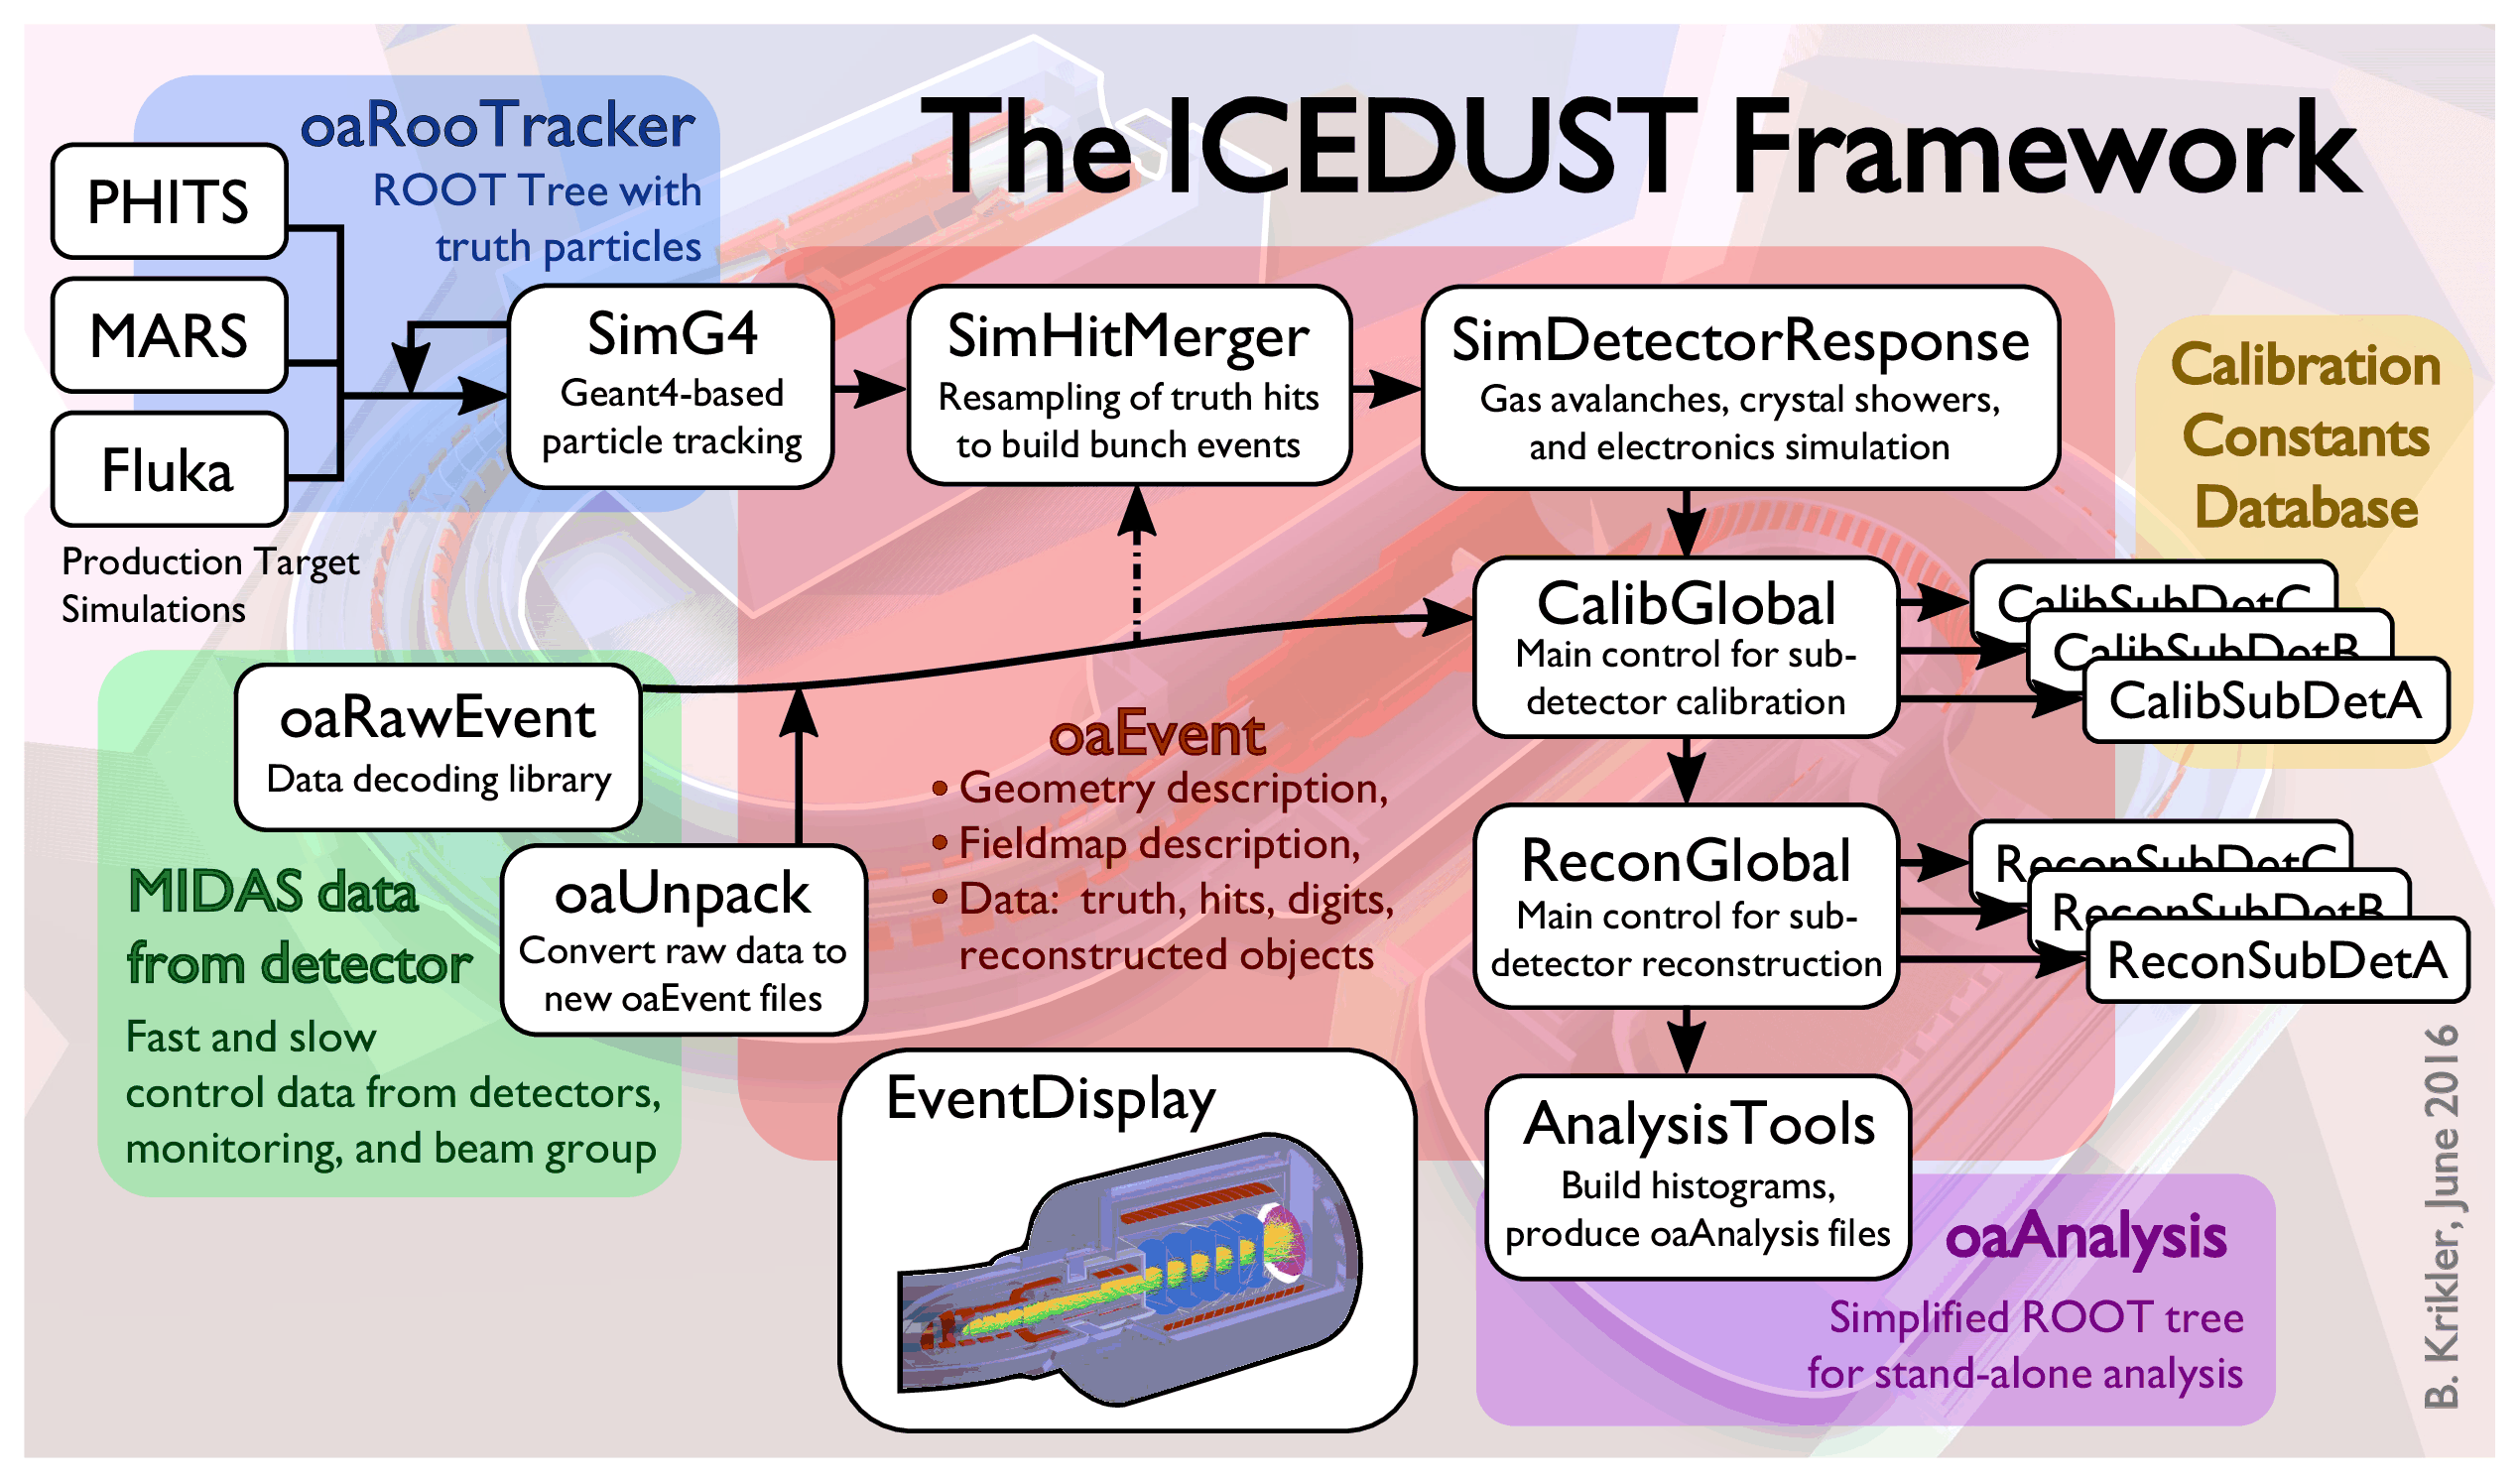
\includegraphics[width=1.00\textwidth,trim=0.85cm 0.5cm 0.5cm 0.5cm,clip=true]{figs/software/ICEDUST_structure}
%}
\caption{
Overview diagram for the ICEDUST framework.
Data produced from simulation or taken in the real experiment are treated identically through the calibration and onwards up to analysis.
}
\figlabel{software:ICEDUSTOverview}
\end{figure}
}

\newcommand{\FigNDTwoEighty}{
\begin{figure}[t]
\centering
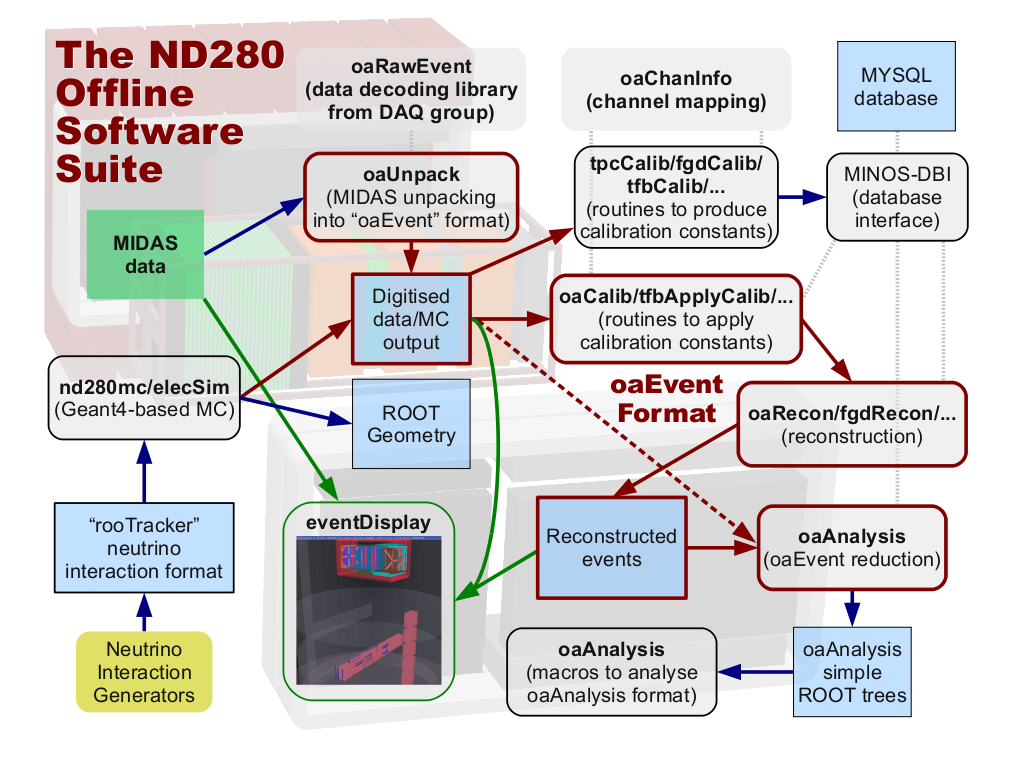
\includegraphics[width=0.95\textwidth]{figs/software/ND280SoftwareDiagram}
\caption{
Overview diagram for the ND280 framework.
}
\figlabel{software:ND280}
\end{figure}
}

\newcommand{\FigSimulationOverview}{
\begin{figure}[t]
\centering
%\fbox{
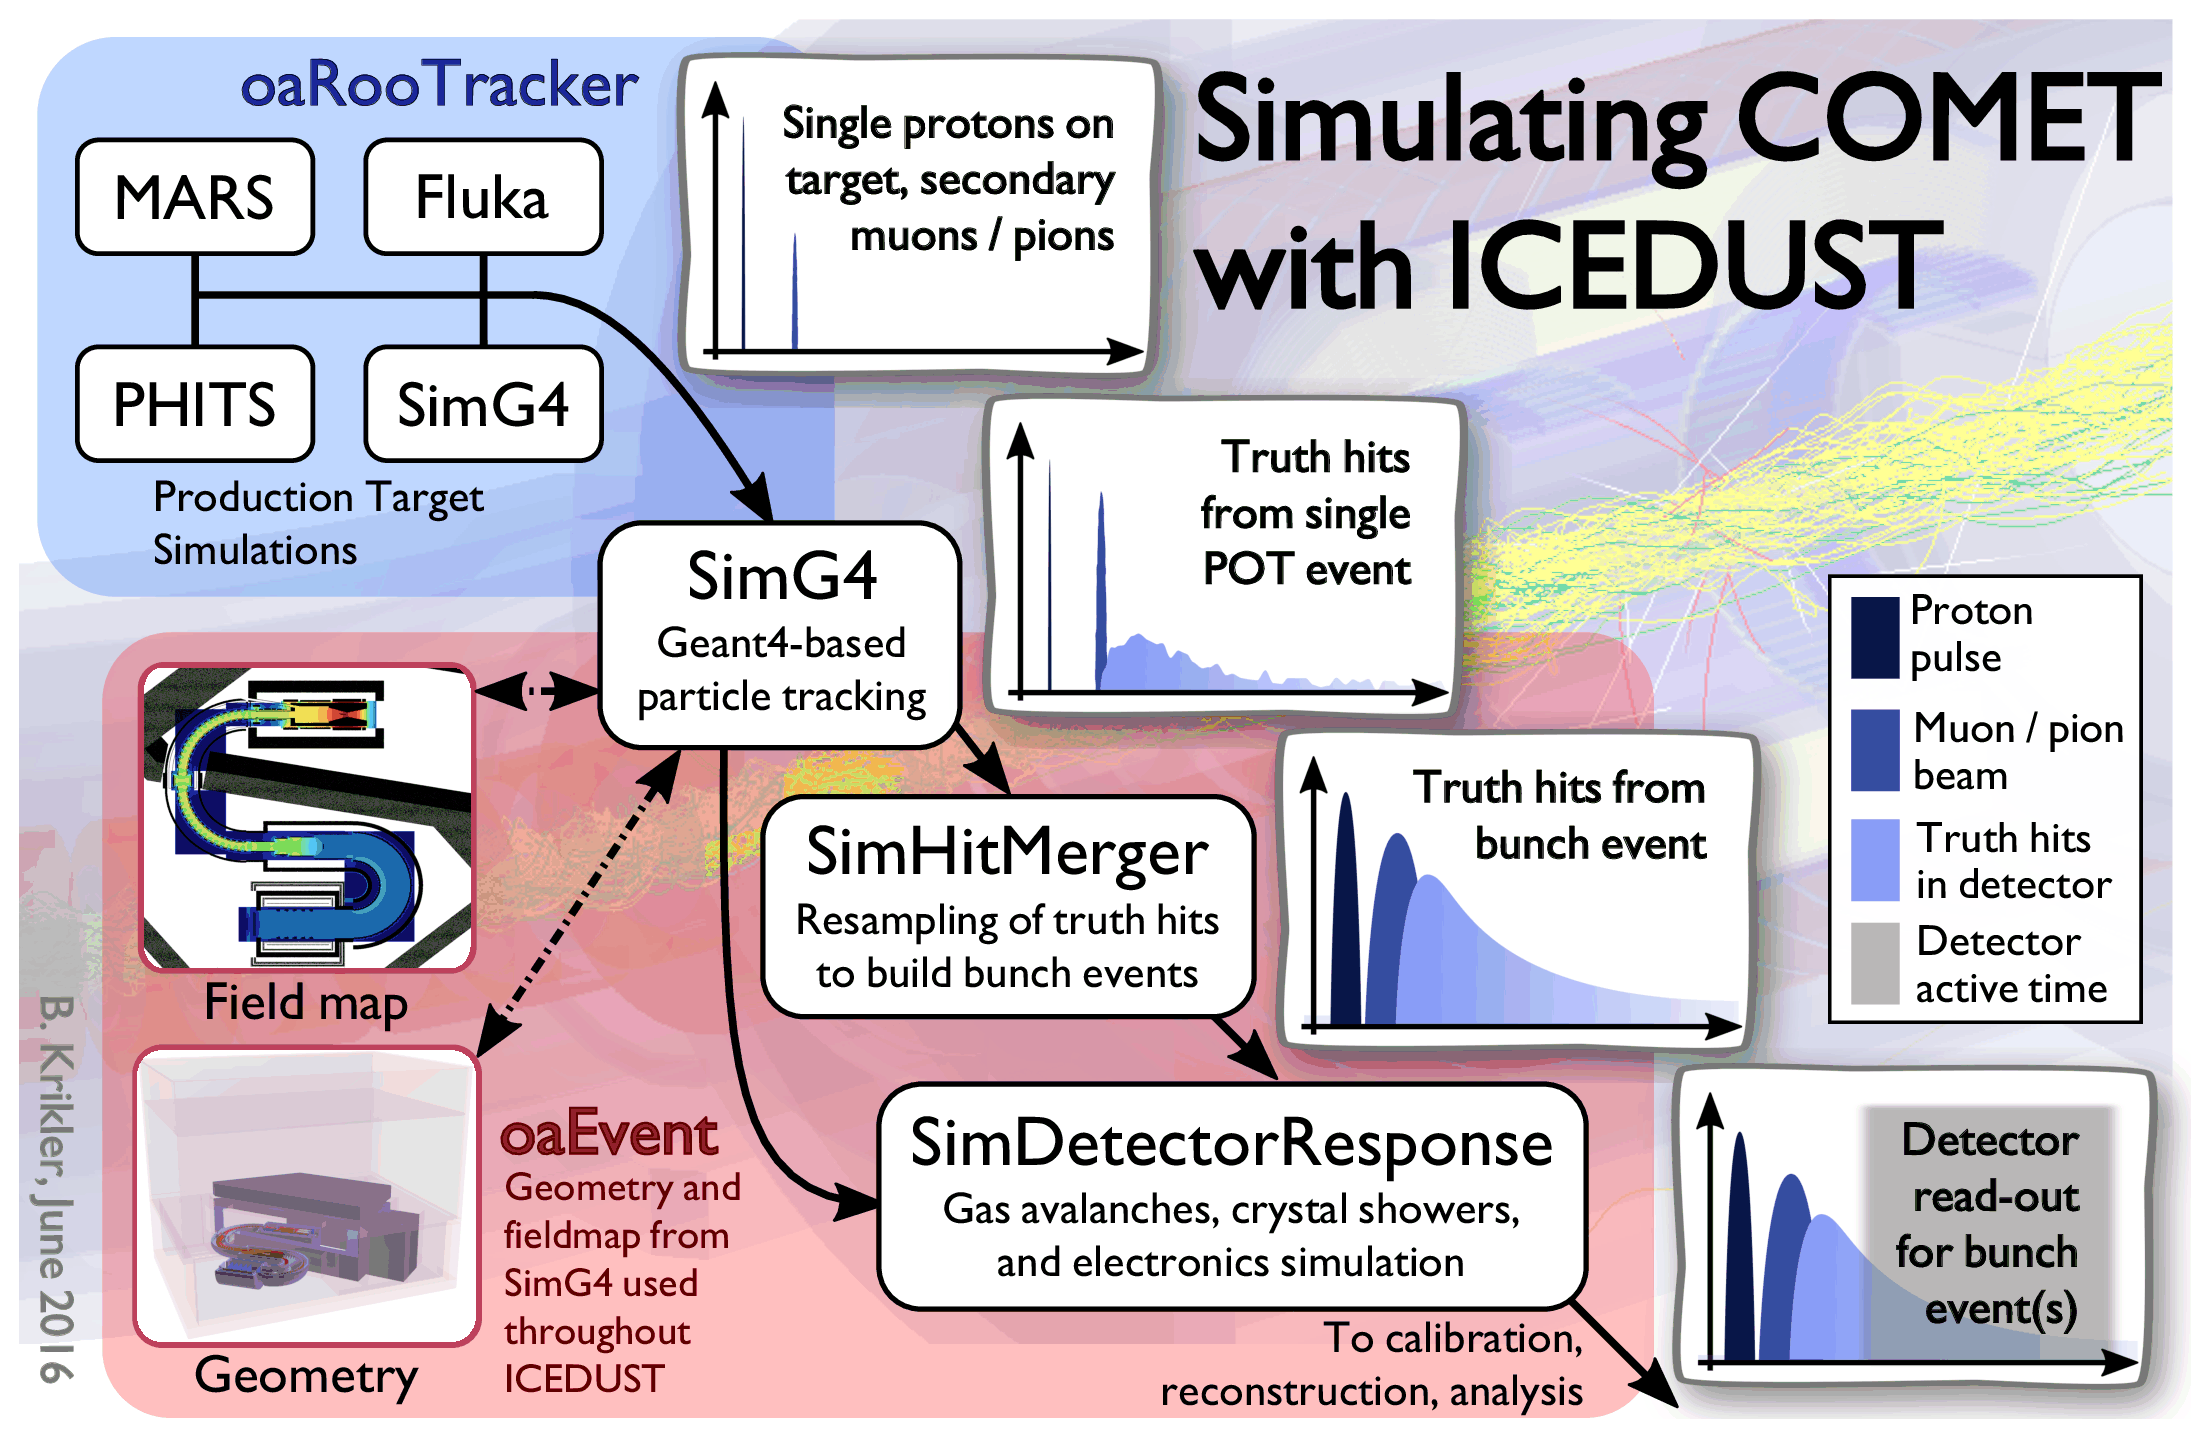
\includegraphics[width=1.00\textwidth]{figs/software/Simulation_structure}
%}
\caption{
Diagram showing the stages used to simulate COMET.
The timing schematics on the right show how a simulated event is built up, firstly by producing many individual proton interactions with the production target,
then by transporting the secondary particles to produce energy deposits in the detector, which are then combined with the truth hits from other proton events to produce a realistic bunch structure.
Finally, these bunch events are processed through the detector response simulation to produce fake waveforms and other detector read-outs.
}
\figlabel{software:SimulationOverview}
\end{figure}
}

\newcommand{\FigGeometryHeirarchy}{
\begin{figure}[t]
\centering
%\fbox{
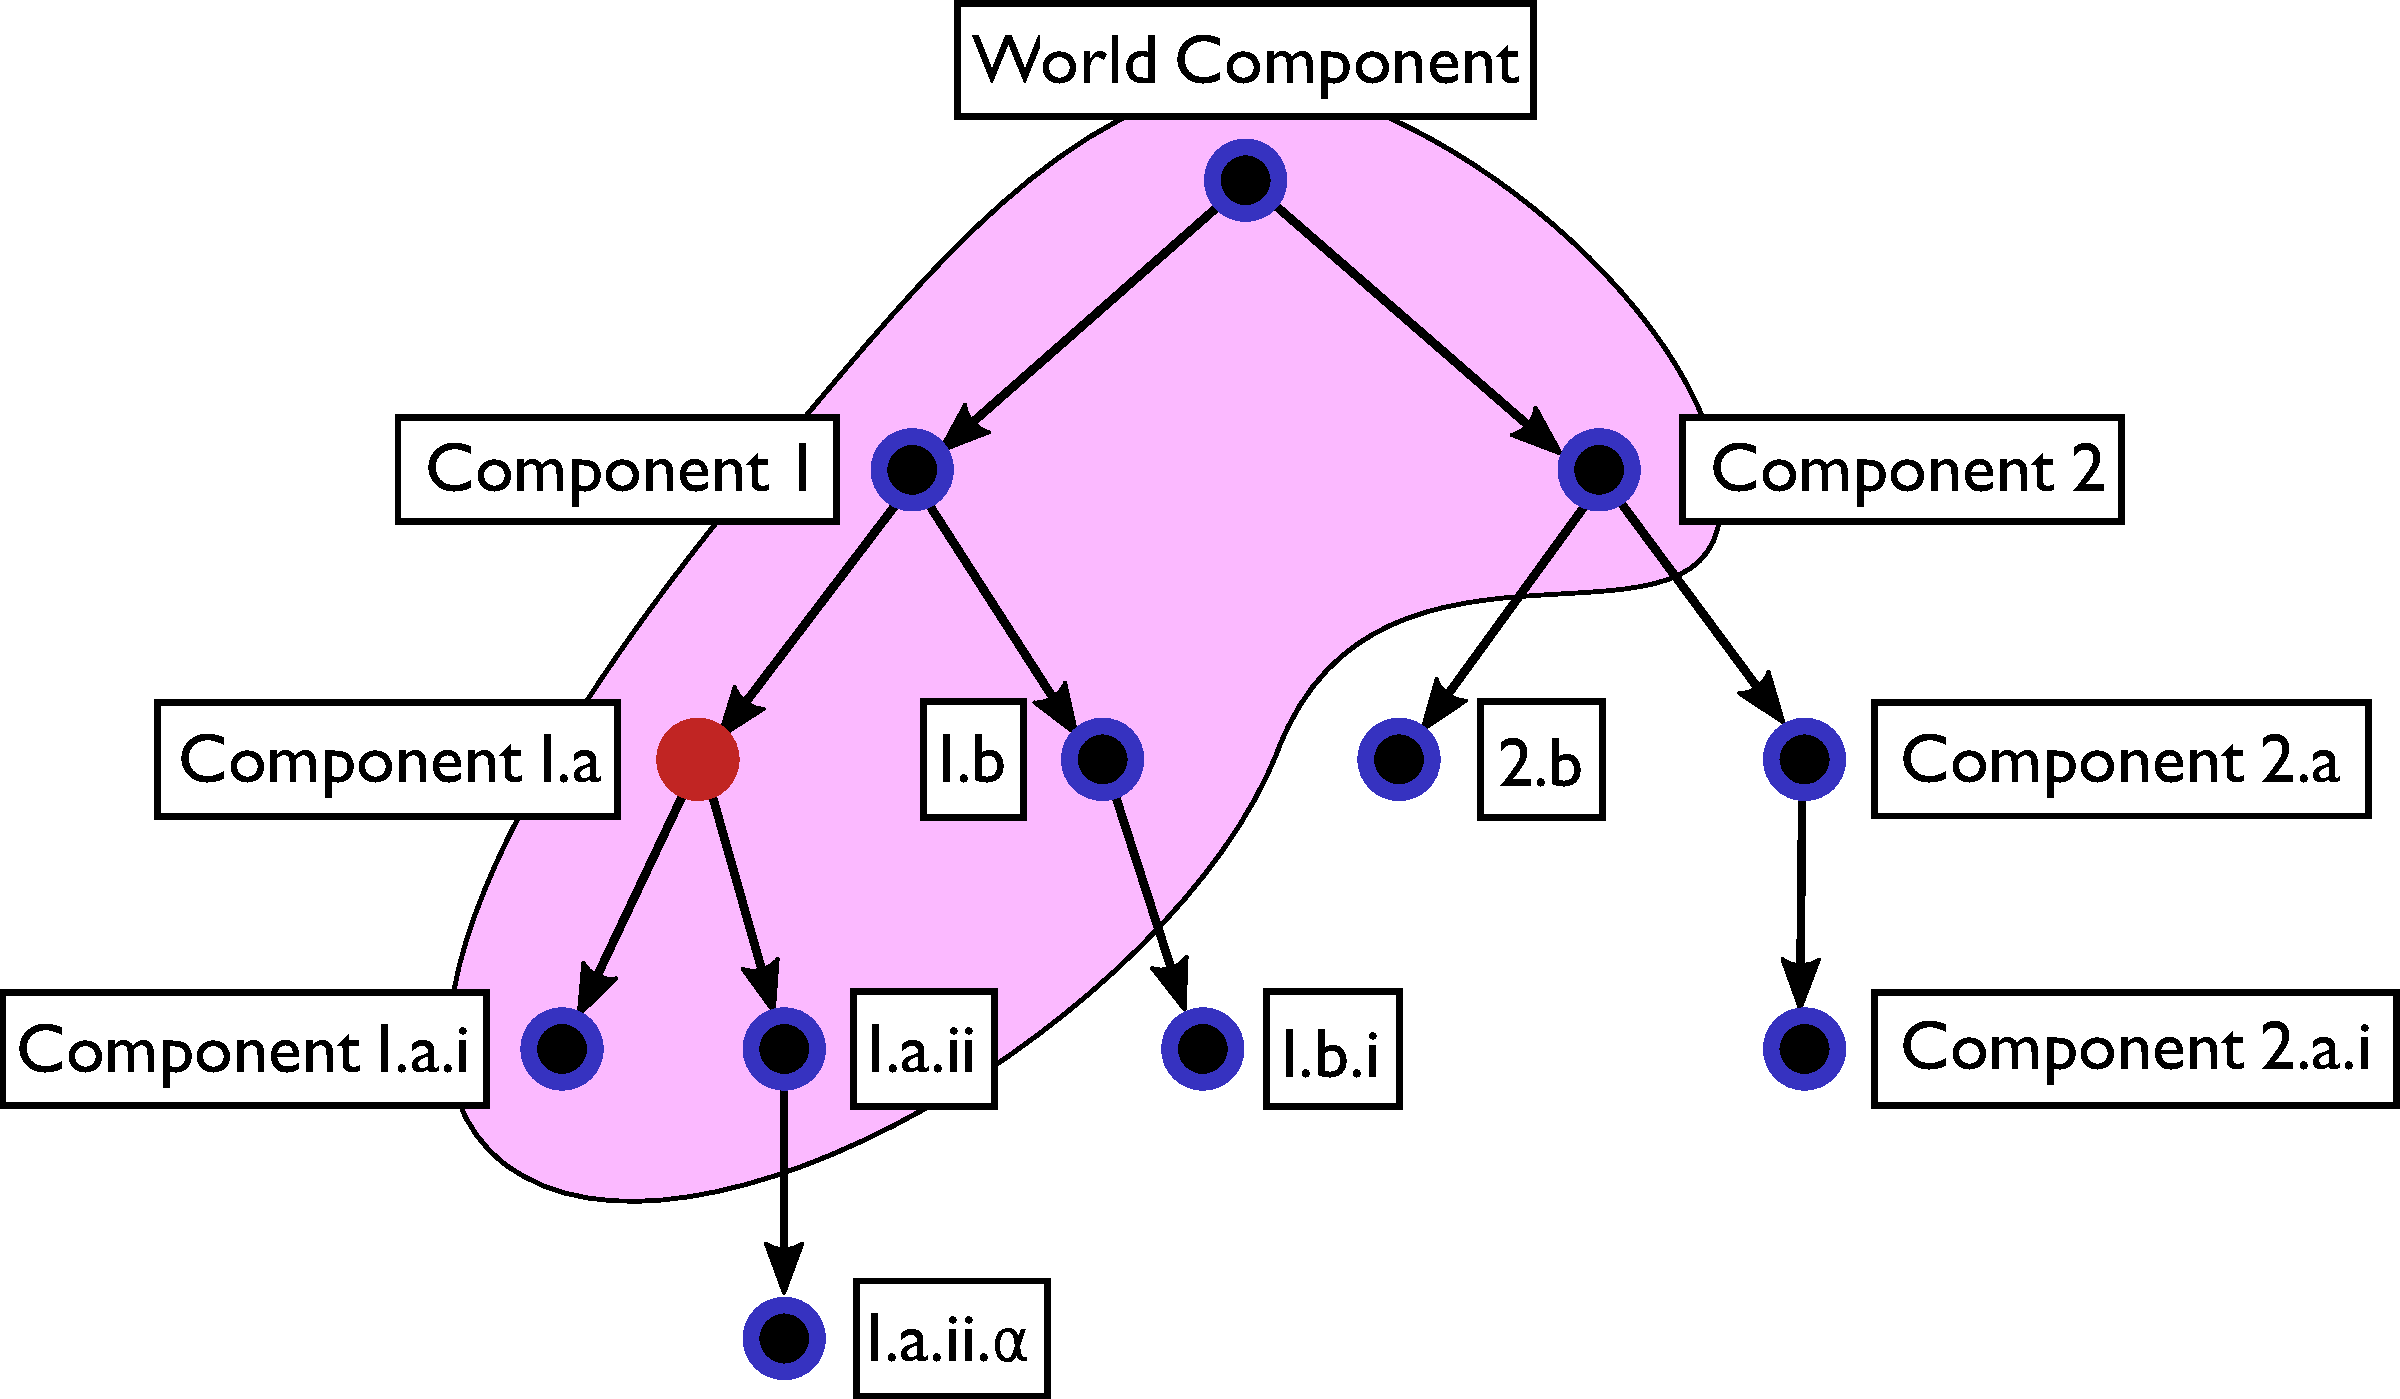
\includegraphics[width=0.70\textwidth]{figs/software/ComponentHeirarchy}
%}
\caption{
How parameters are shared amongst different components.
Parameters of component 1.a (in red) can access the value of parameters owned by components contained in the larger violet region.
}
\figlabel{software:componentHeirarchy}
\end{figure}
}

\newcommand{\FigGeometryParameters}{
\begin{figure}[t]
\lstinputlisting[style=customc]{figs/software/demo-parameters.mac}
\caption{
An example set of parameter definitions which control the geometry for the Torus2.
Parameter specifications use natural arithmetic notation and can reference other parameters and use standard units.
They can also be formed as sets where each element has a different value, such as the \texttt{Coils:Position} parameter.
}
\figlabel{software:geom:paramAssignments}
\end{figure}
}

\newcommand{\FigGeometryScreenshots}{
\begin{figure}[tb]
        \subfloat[][\figlabel{software:geom:screenshots:phaseI}\phaseI]  {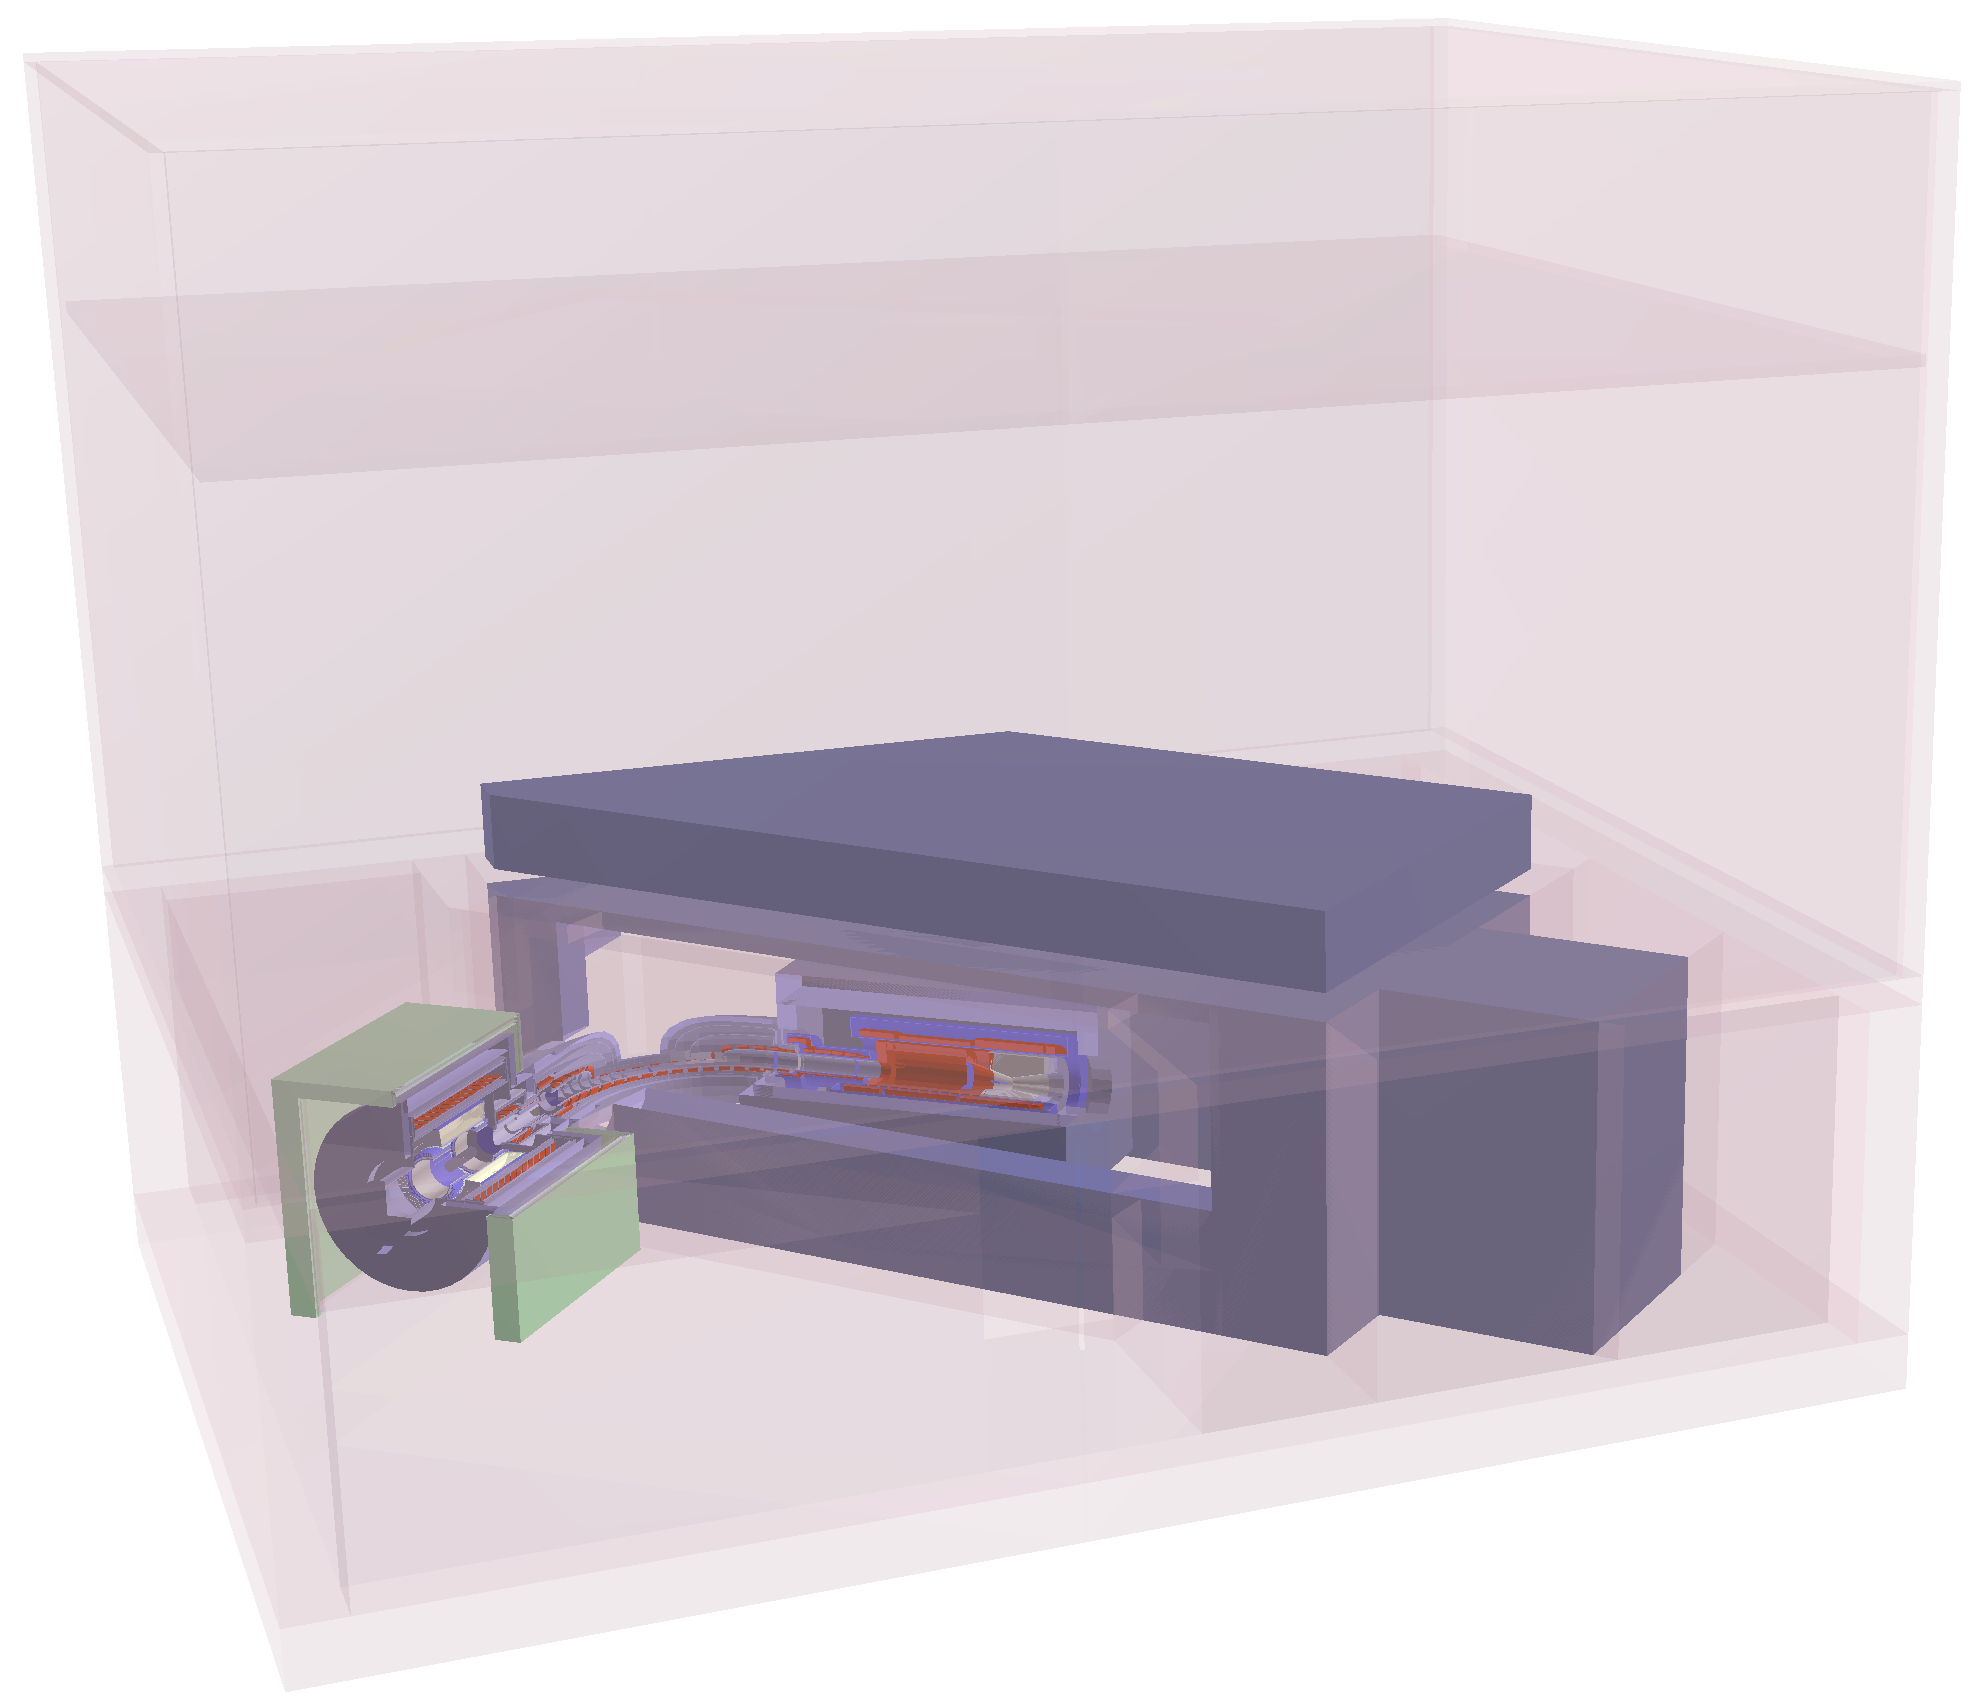
\includegraphics[height=0.25\textheight]{figs/software/Phase-I-UpdateGeom}}\hspace{2ex}%
        \subfloat[][\figlabel{software:geom:screenshots:phaseII}\phaseII]{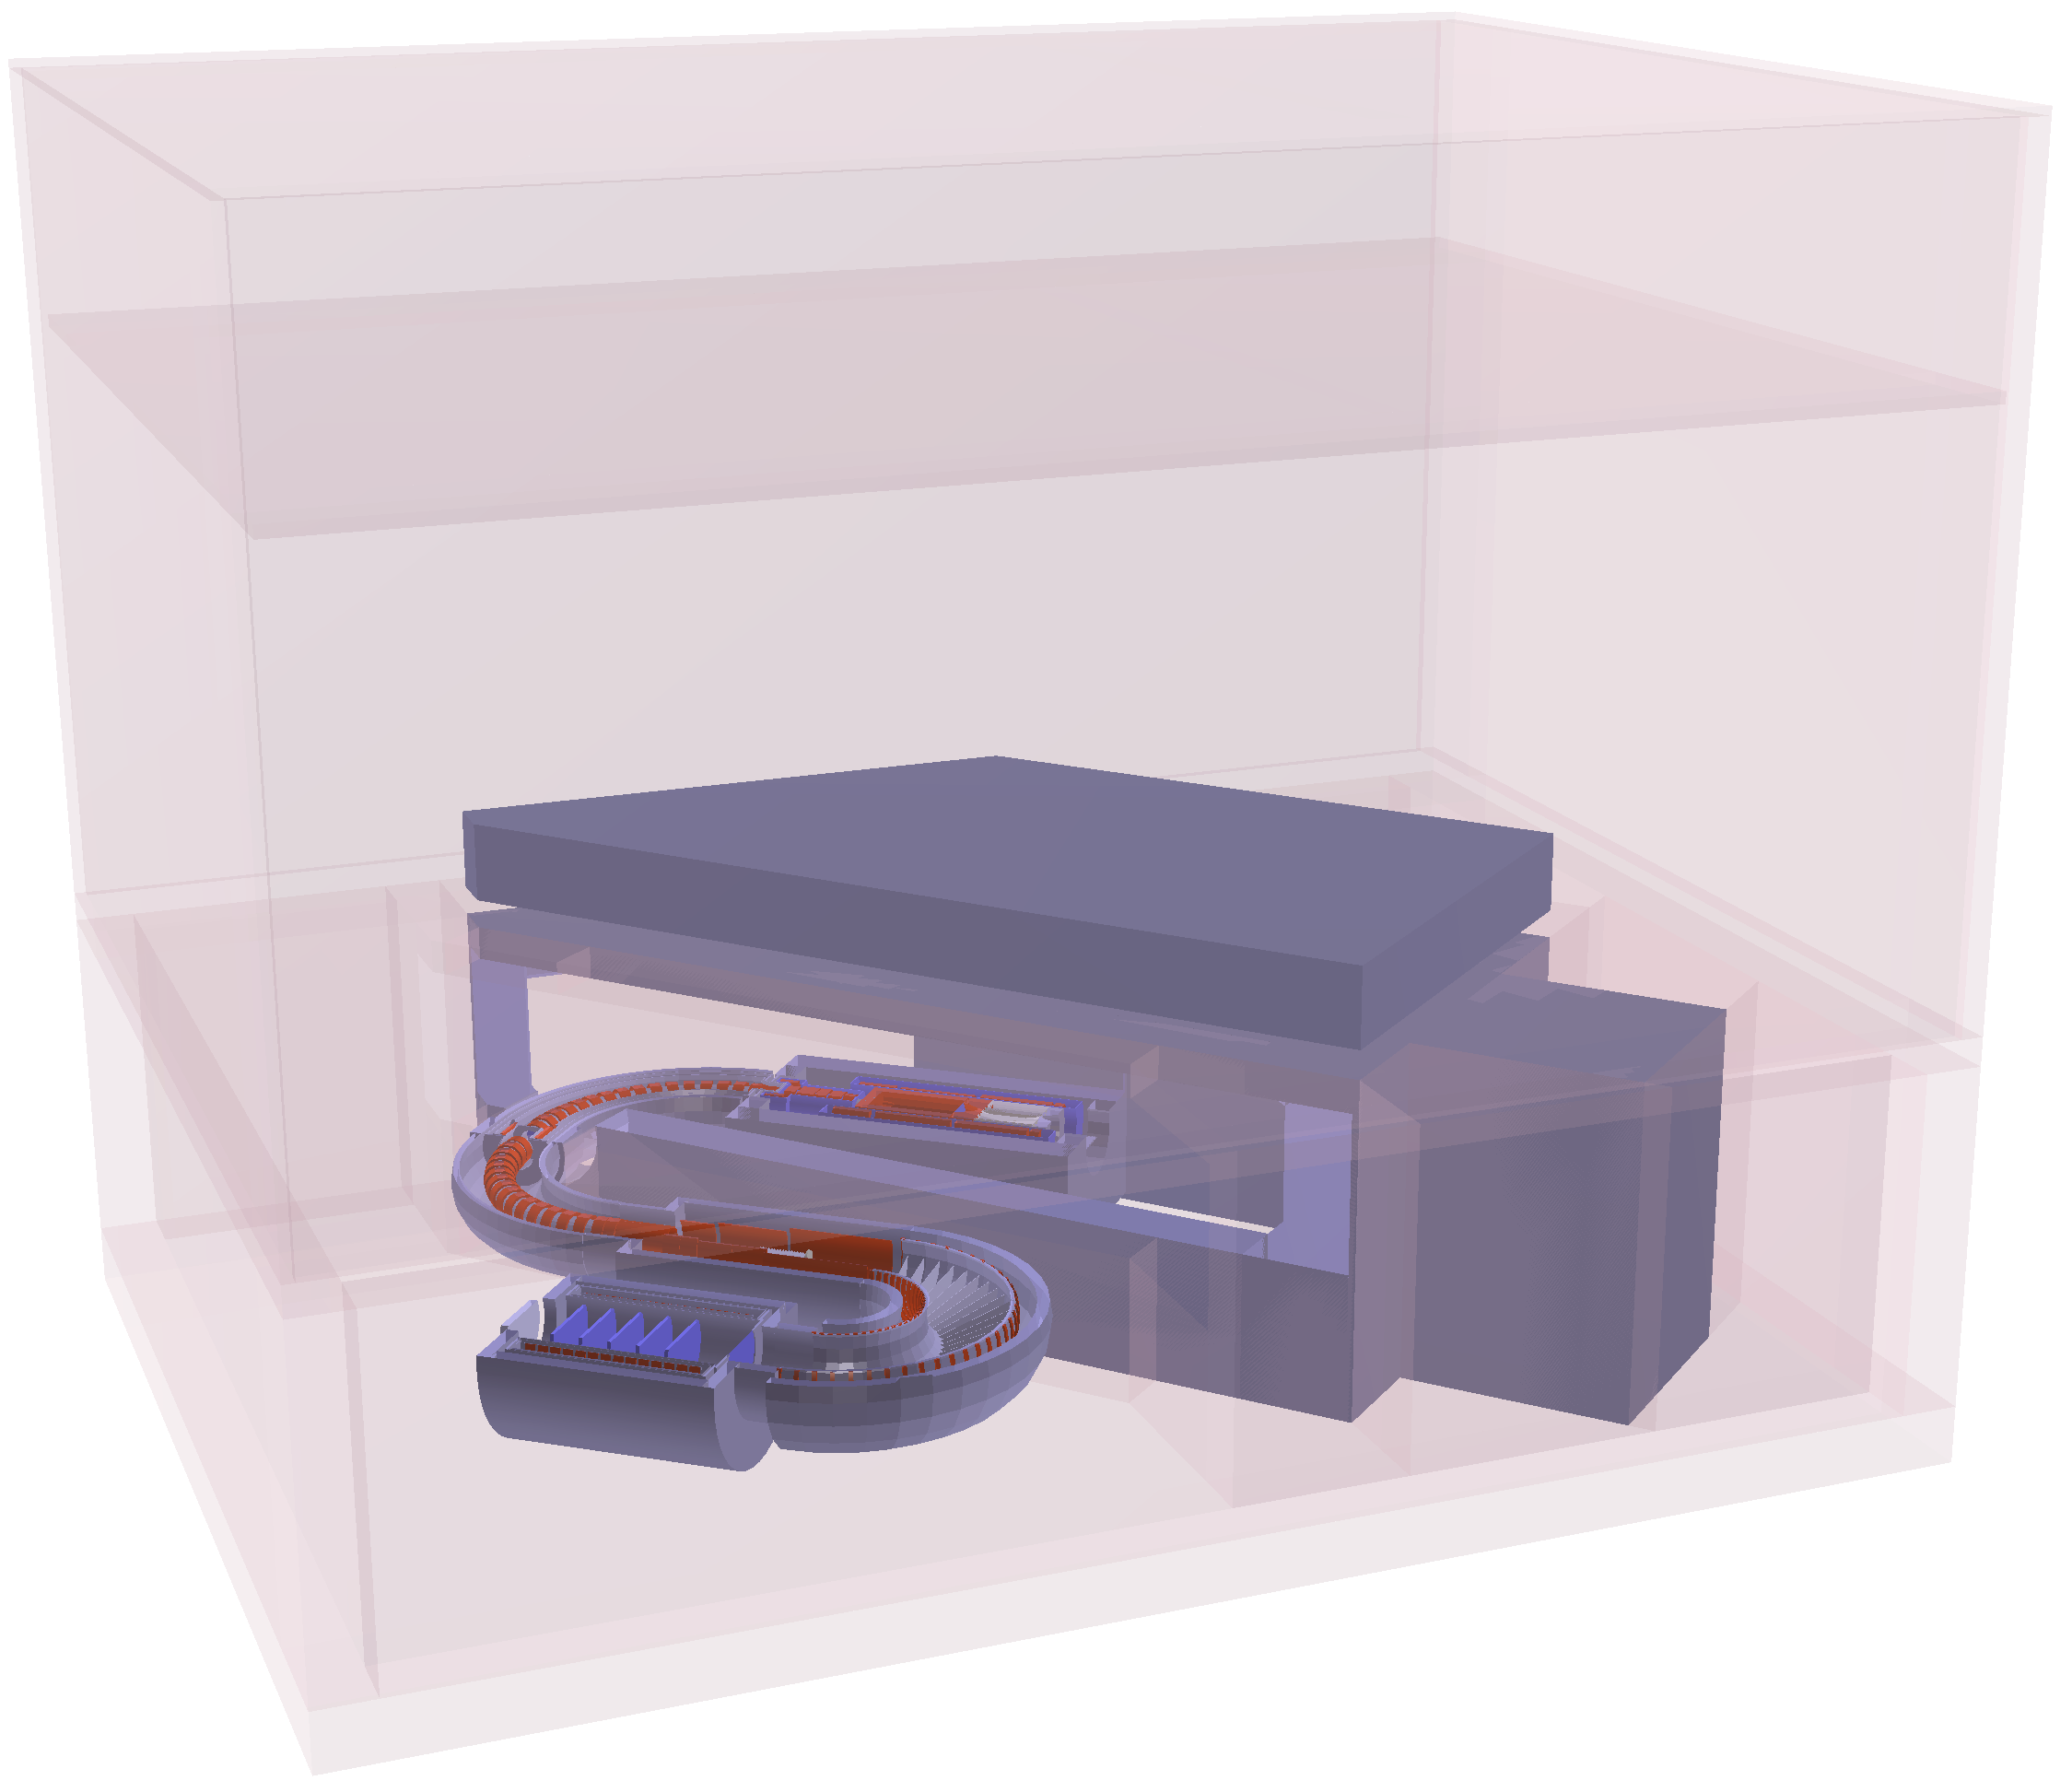
\includegraphics[height=0.25\textheight,trim=0 0.3cm 0 2.6cm,clip=true]{figs/software/Phase-II-UpdateGeom.png}}
\caption{\figlabel{software:geom:screenshots} %
Two of the possible simulation `worlds' that can be selected at run-time:
        \protect\subref{fig:software:geom:screenshots:phaseI} \phaseI with the CyDet detector installed, and
        \protect\subref{fig:software:geom:screenshots:phaseII} \phaseII.  
	Mutiple \phaseI worlds exist, one for each potential running configuration.
}
\end{figure}
}

\newcommand{\FigPiYieldHadronCodes}{
\begin{figure}[b]
\centering
%\fbox{
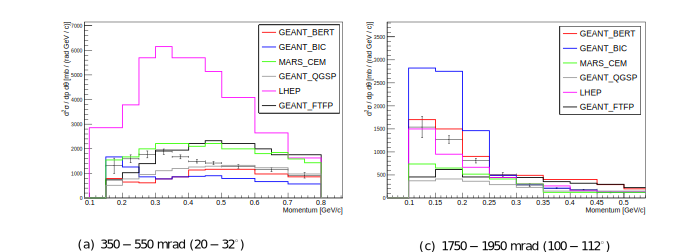
\includegraphics[width=0.95\textwidth,trim=2cm 1cm 0.8cm 0.5cm,clip=true]{figs/software/PionYield_AEdmondsThesis}
%}
\caption{
Comparison of various hadron production codes with experimental data from the HARP experiment, taken from the thesis of A. Edmonds~\cite{AEdmondsThesis}.
Points with error bars are the experimental data.  Left: double differential-production cross-section for pion production from 20 to 32\degree with respect to the incoming proton direction; right: from 100 to 112\degree.
The hadron production code that best reproduces the data depends strongly on the angular region under consideration.
}
\figlabel{software:piYield}
\end{figure}
}

\newcommand{\FigSoftwarePhysicsSpectra}{
\begin{figure}[p]
\centering
%\fbox{
\subfloat[][\figlabel{software:customPhysic:DIO}Electrons from $\mu$ Decay-in-Orbit]{
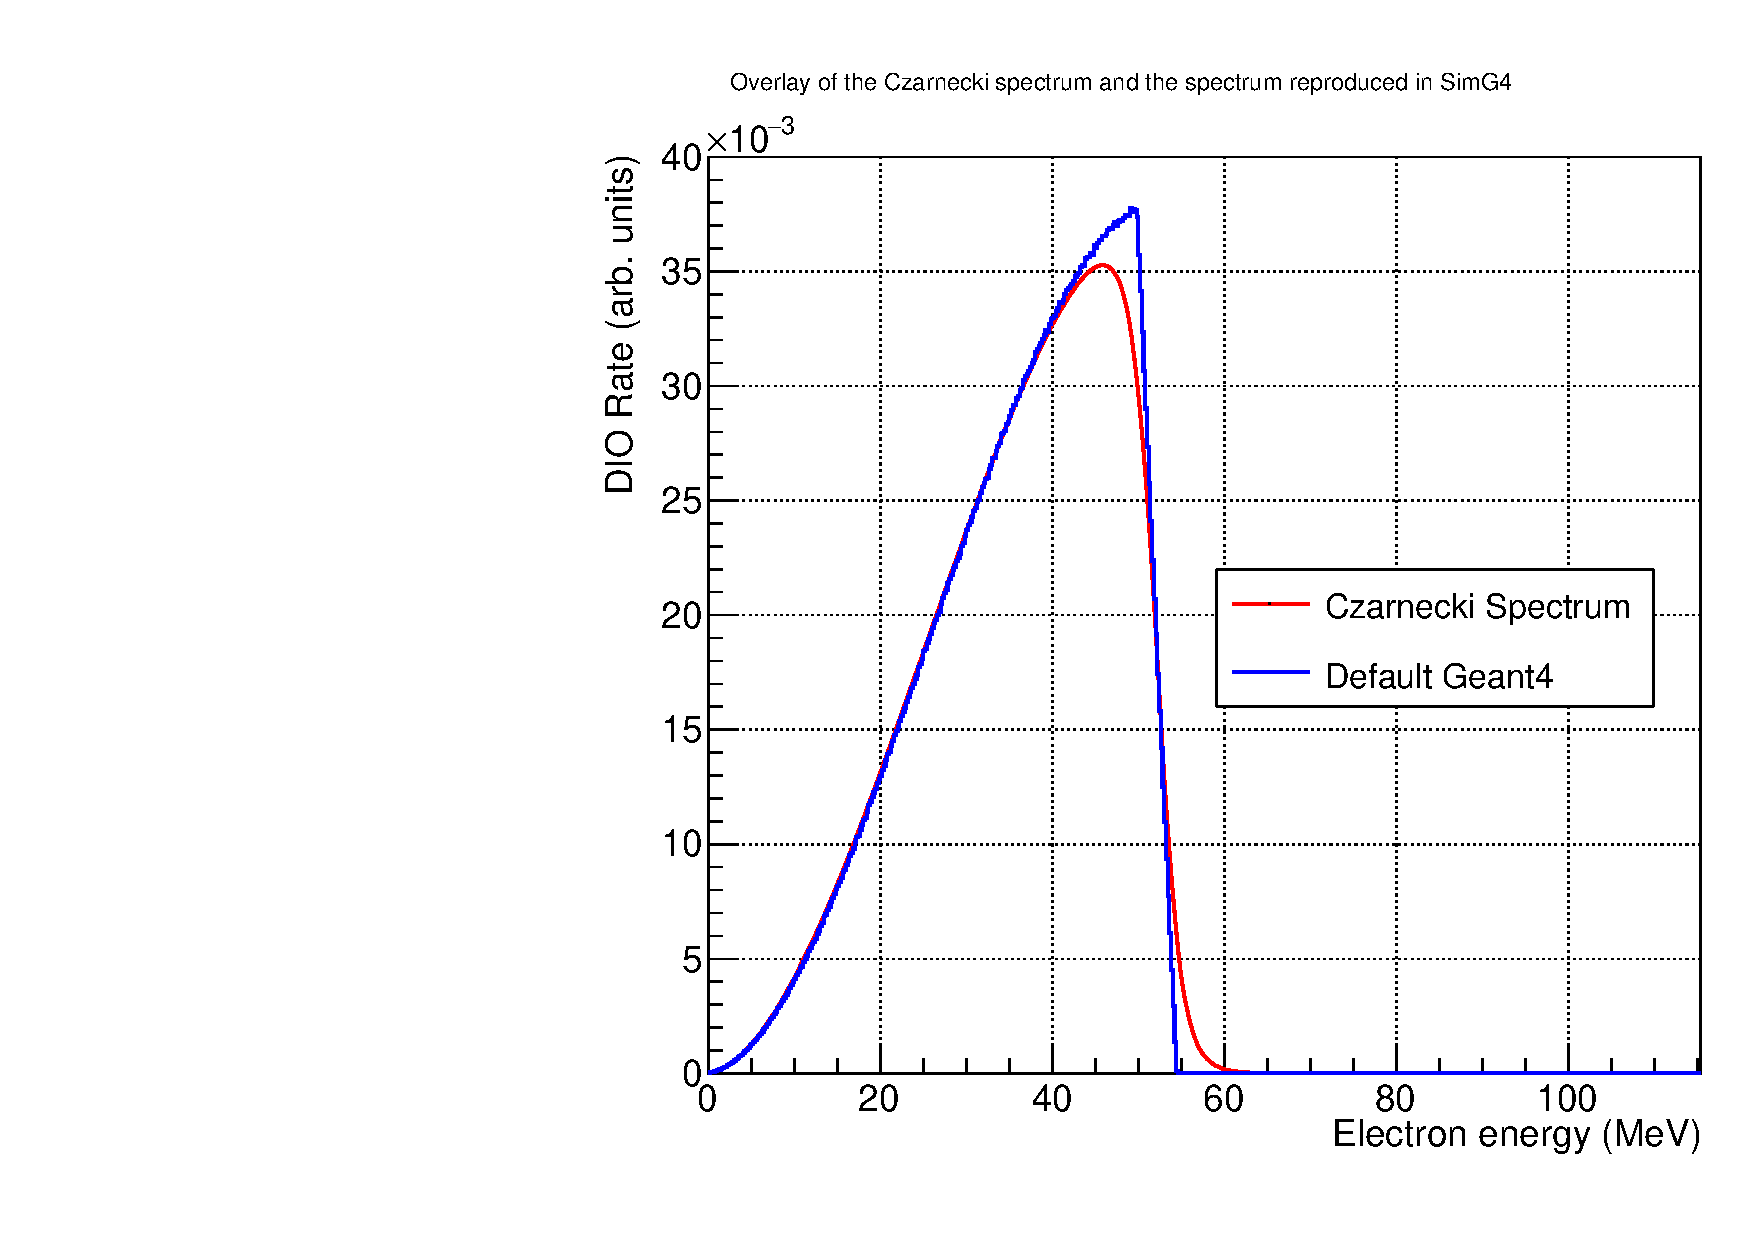
\includegraphics[width=0.45\textwidth,trim=0cm 0cm 0.0cm 1.3cm,clip=true]{figs/software/160822_BoundDecay_Geant4_vs_Czarnecki-lin.pdf}
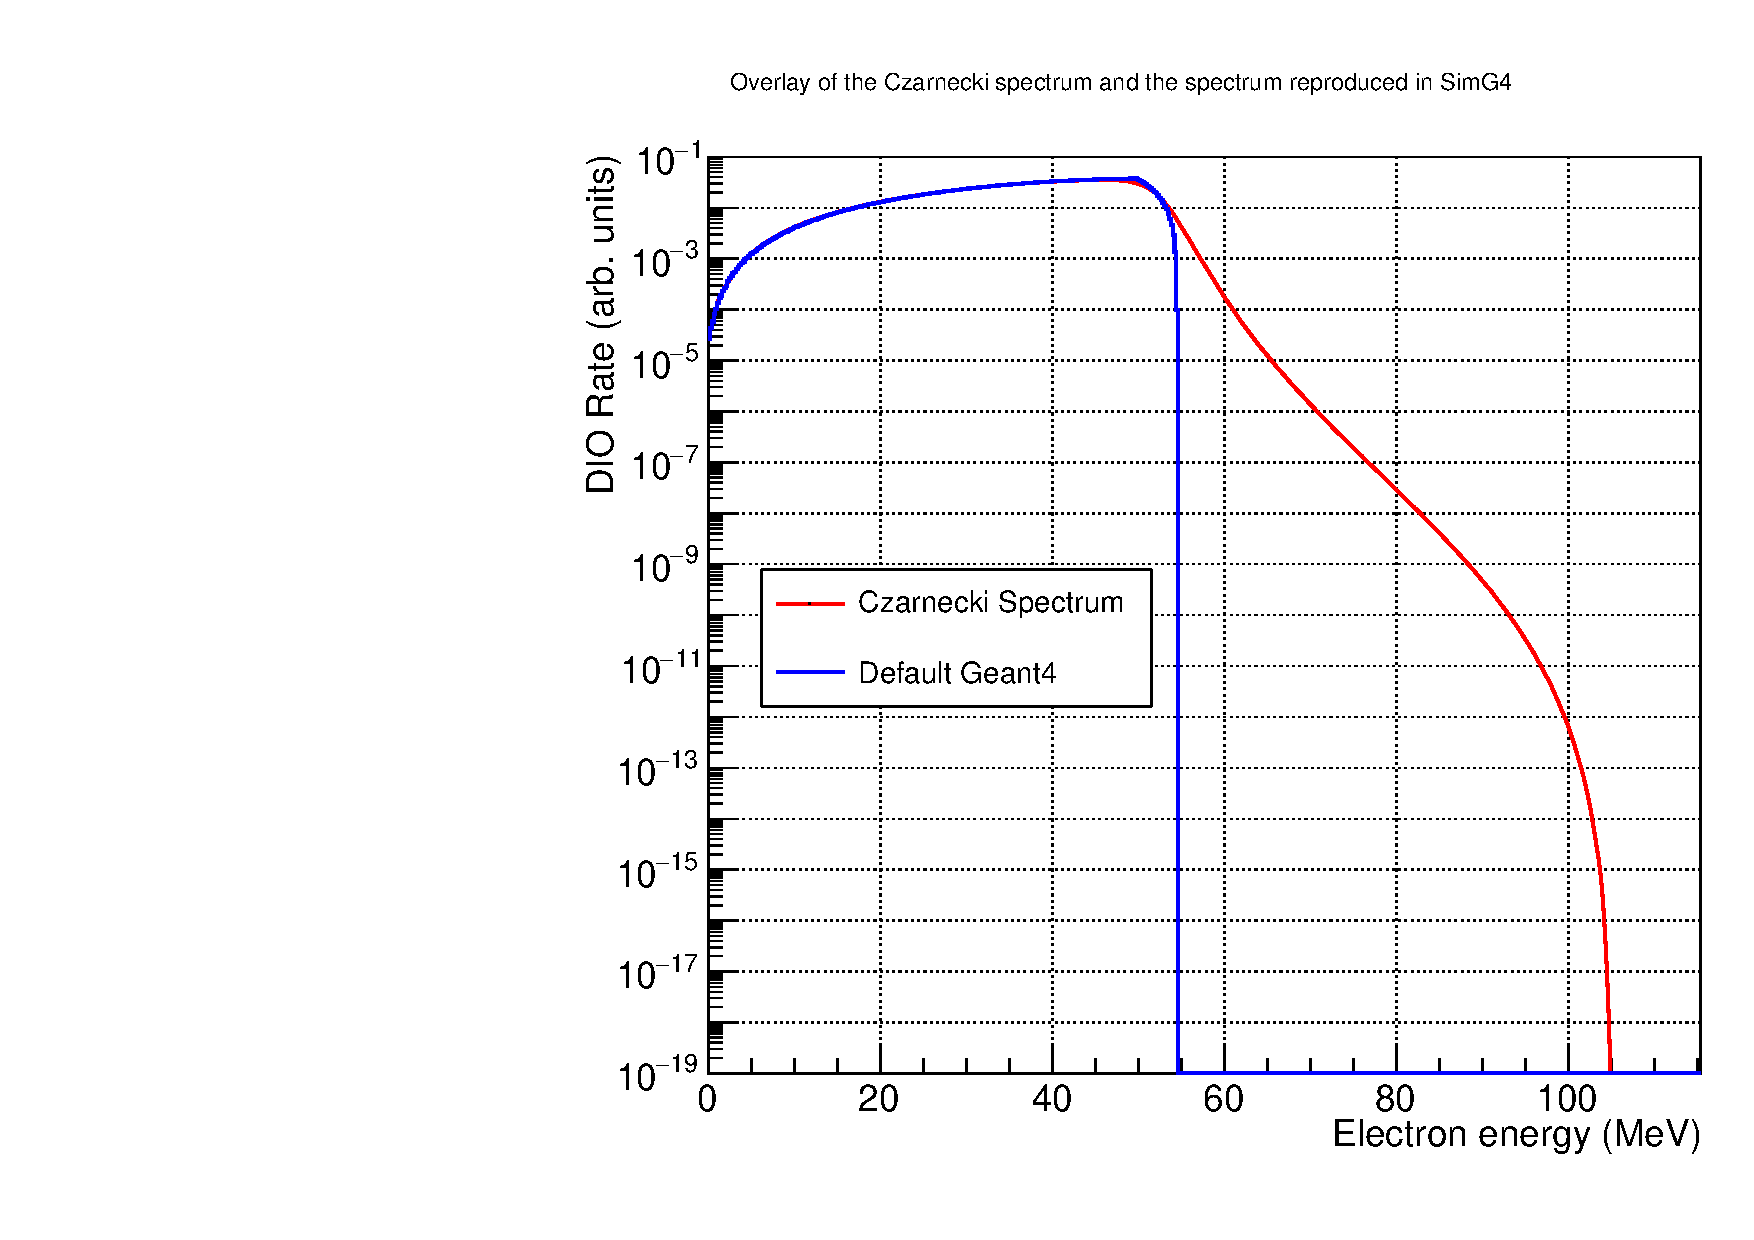
\includegraphics[width=0.45\textwidth,trim=0cm 0cm 0.0cm 1.3cm,clip=true]{figs/software/160822_BoundDecay_Geant4_vs_Czarnecki-log.pdf}
}\\
\subfloat[][\figlabel{software:customPhysic:ProtMuCap}Protons Emitted Following $\mu$ Nuclear Capture]{
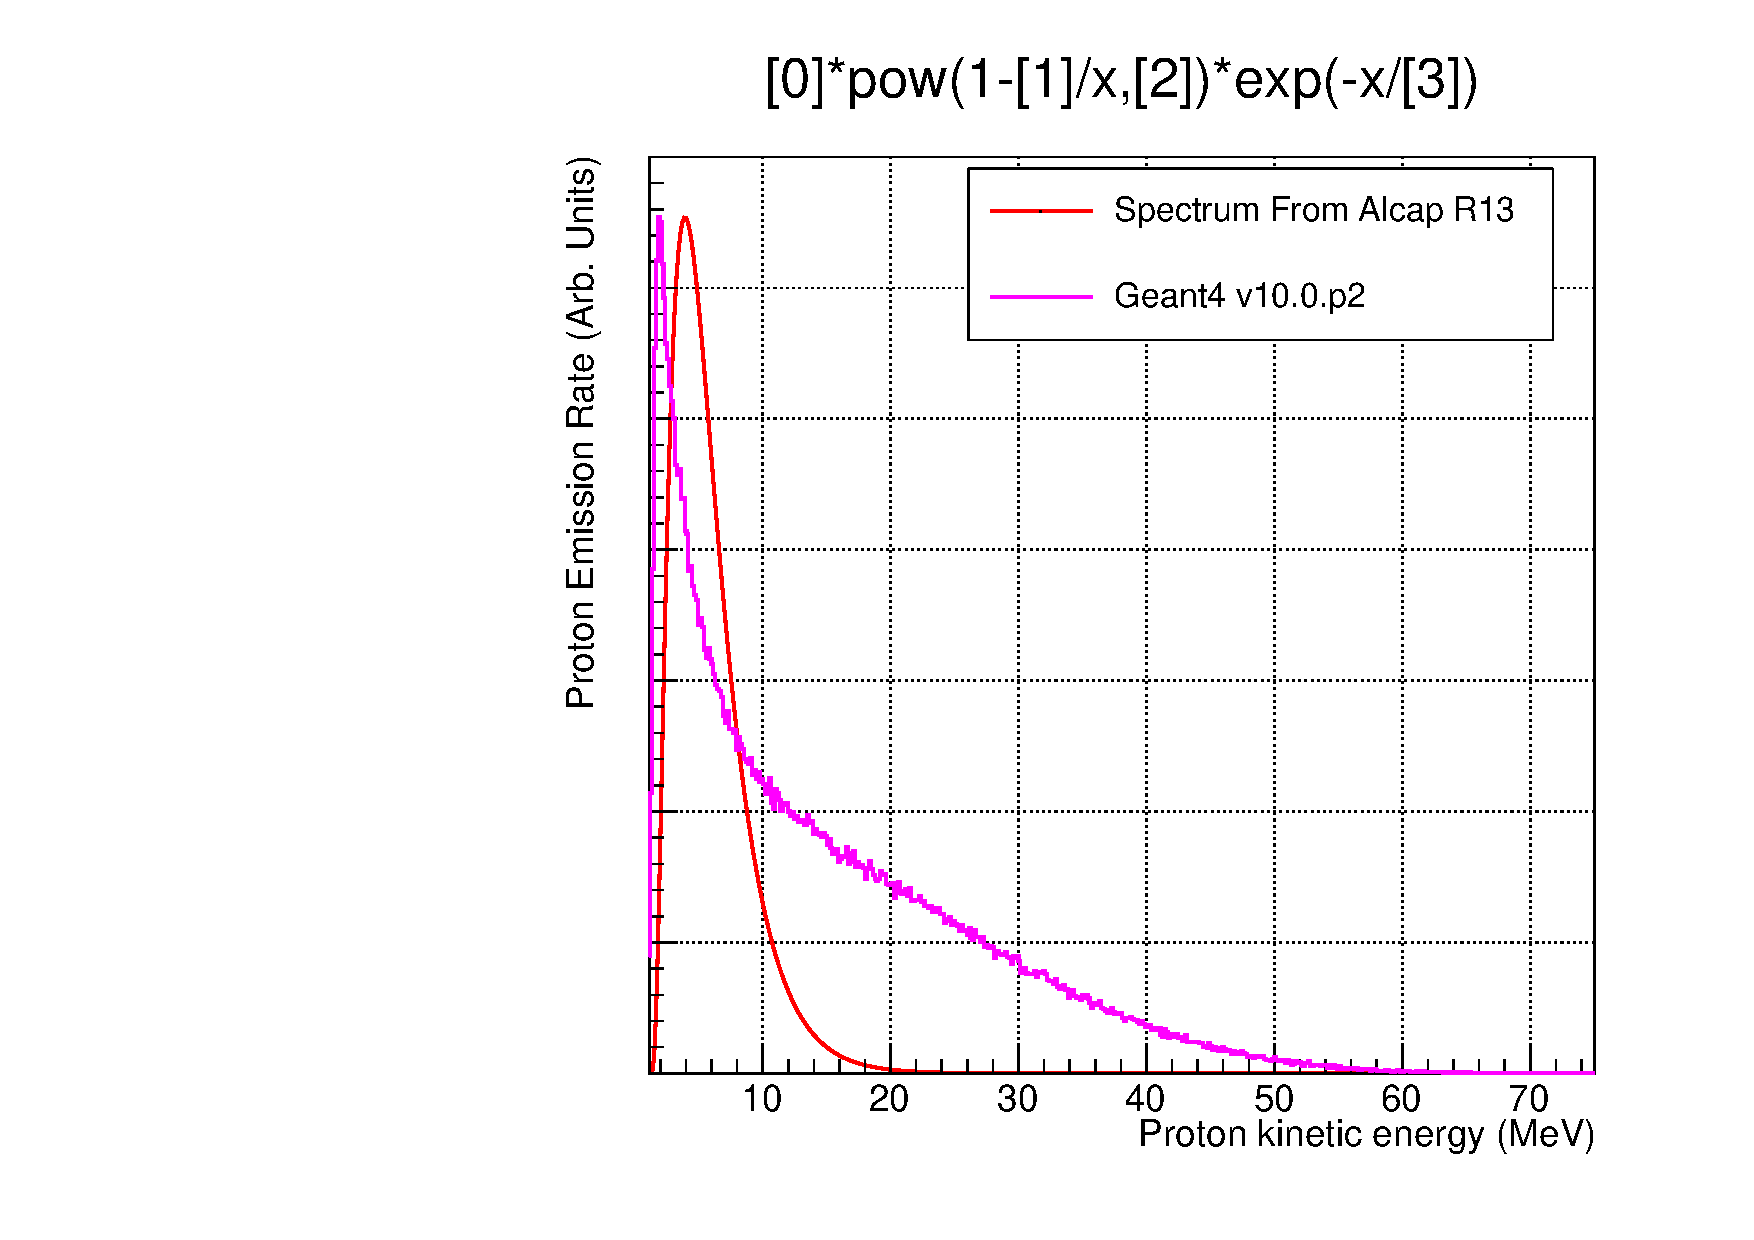
\includegraphics[width=0.45\textwidth,trim=0cm 0cm 1.8cm 1.9cm,clip=true]{figs/software/160822_Geant4VsAlcap-lin.pdf}
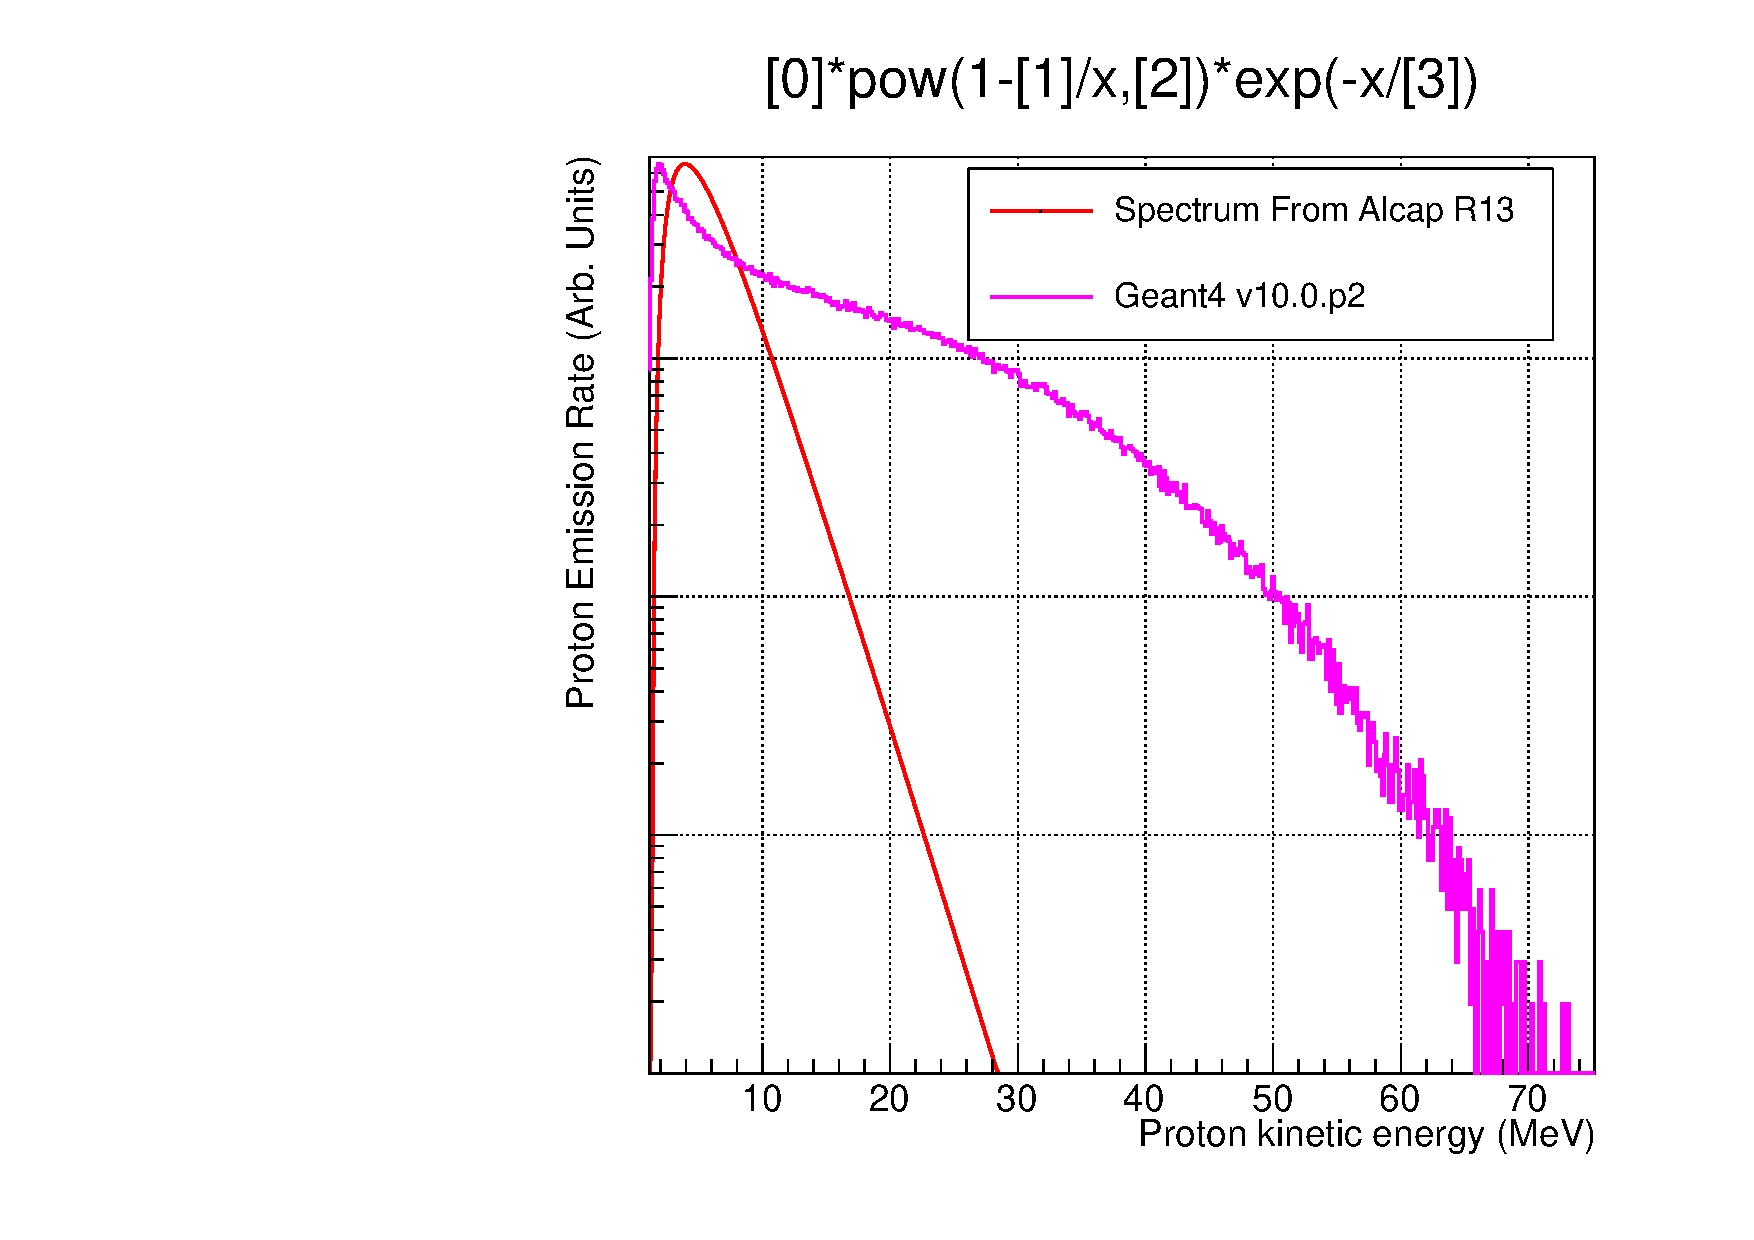
\includegraphics[width=0.45\textwidth,trim=0cm 0cm 1.8cm 1.9cm,clip=true]{figs/software/160822_Geant4VsAlcap-log.pdf}
}
%}
\caption{
\figlabel{software:customPhysic}
Comparison of the realistic spectra for \ac{DIO} electrons, \protect\subref{fig:software:customPhysic:DIO} (normalised to agree at 35~MeV), and protons coming from muon nuclear capture, \protect\subref{fig:software:customPhysic:ProtMuCap} (normalised to have the same maximum value), each on a linear scale (left) and a logarithmic scale (right).
The \ac{DIO} spectrum used in default Geant4 has a sharp cut-off slightly above the free muon decay end-point, to be compared with the long but steeply falling tail of the Czarnecki \etal theoretical calculation~\cite{Czarnecki2011}.
The comparison of protons coming from muon capture between the preliminary result from AlCap and default Geant4 shows that the true proton spectrum is much softer than the Geant4 model.
}
\end{figure}
}

\newcommand{\FigSimulationPhysicsClasses}{
\begin{figure}[tb]
\centering
%\fbox{
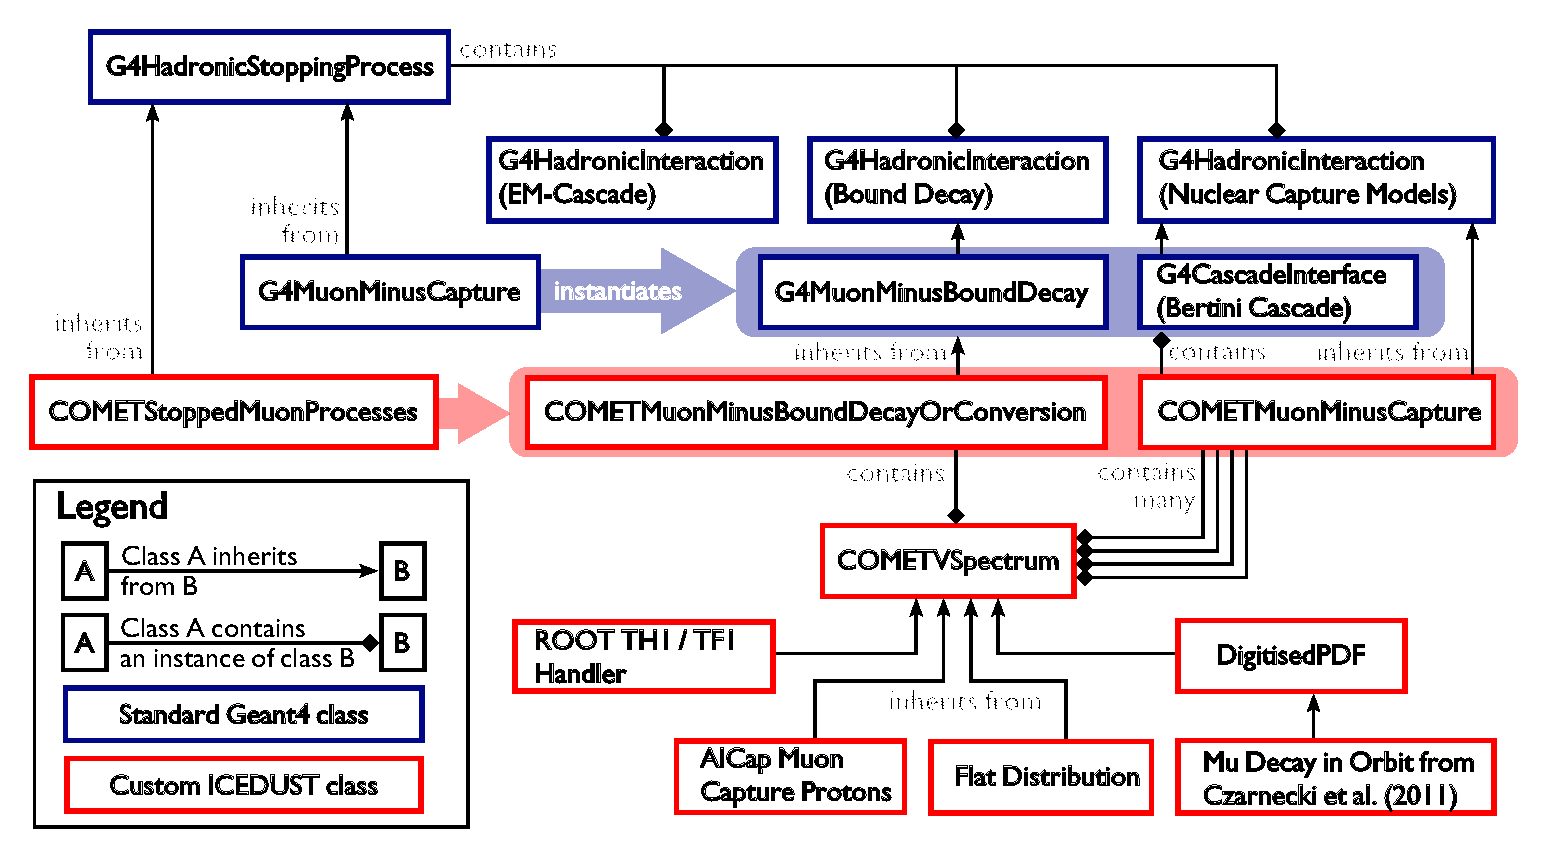
\includegraphics[width=1.00\textwidth]{figs/software/SimulationMuonPhysicsClasses}
%}
\caption{
The various classes involved in simulating the various processes of stopped negative muons.
%Classes in red have been implemented for COMET and augment the existing Geant4 classes which are shown in blue.
The standard Geant4 model is activated by registering `G4MuonMinusCapture', which instantiates `G4MuonMinusBoundDecay' and `G4CascadeInterface' to run the \ac{DIO} and nuclear capture respectively.
To use the custom COMET muon physics, an instance of `COMETStoppedMuonProcess' should be registered, which sets up `COMETMuonMinusBoundDecayOrConversion' to produce the electron (and possibly neutrinos) from \ac{DIO} or conversion, and `COMETMuonMinusCapture' to do the nuclear capture.
}
\figlabel{software:ExtendedMuonClasses}
\end{figure}
}

\newcommand{\FigSoftwareFieldMap}{
\begin{figure}[b]
\centering
%\fbox{
\subfloat[][\figlabel{software:field:Opera}Opera calculation]{
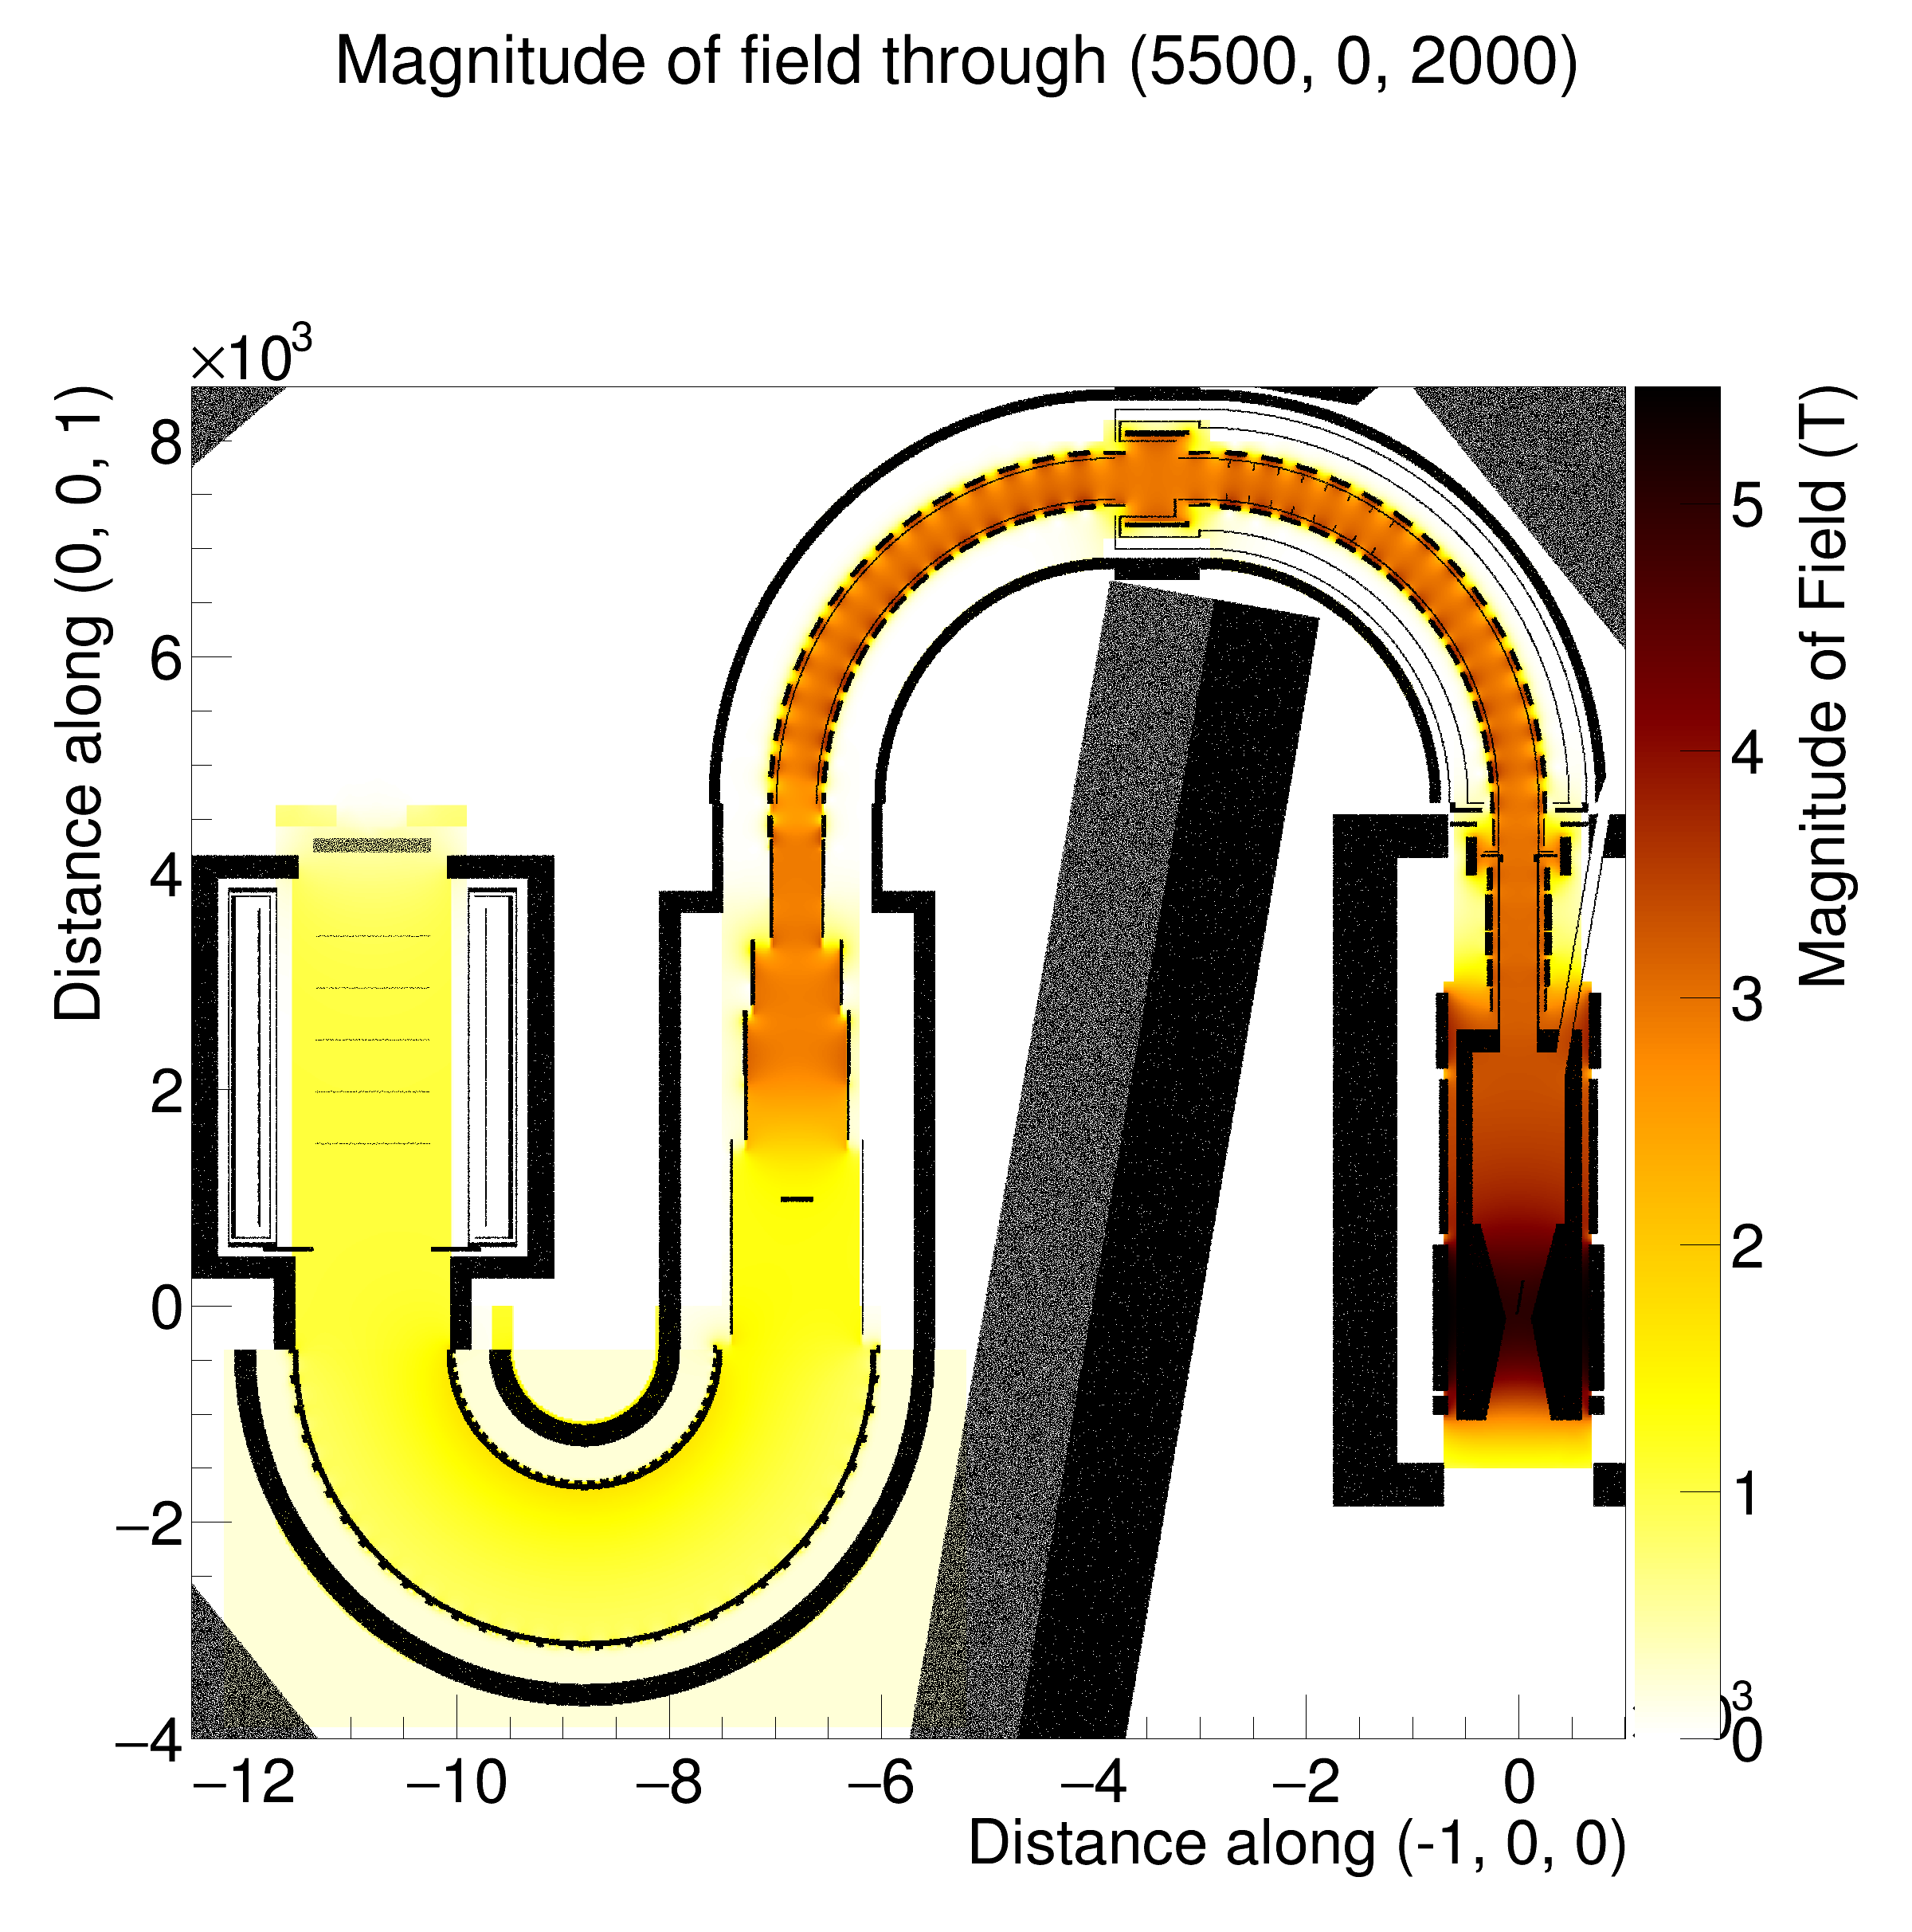
\includegraphics[width=0.45\textwidth,trim=0cm 0cm 0.0cm 13cm,clip=true]{figs/software/Plot_Opera.png}
}
\subfloat[][\figlabel{software:field:G4Beamline}G4Beamline calculation]{
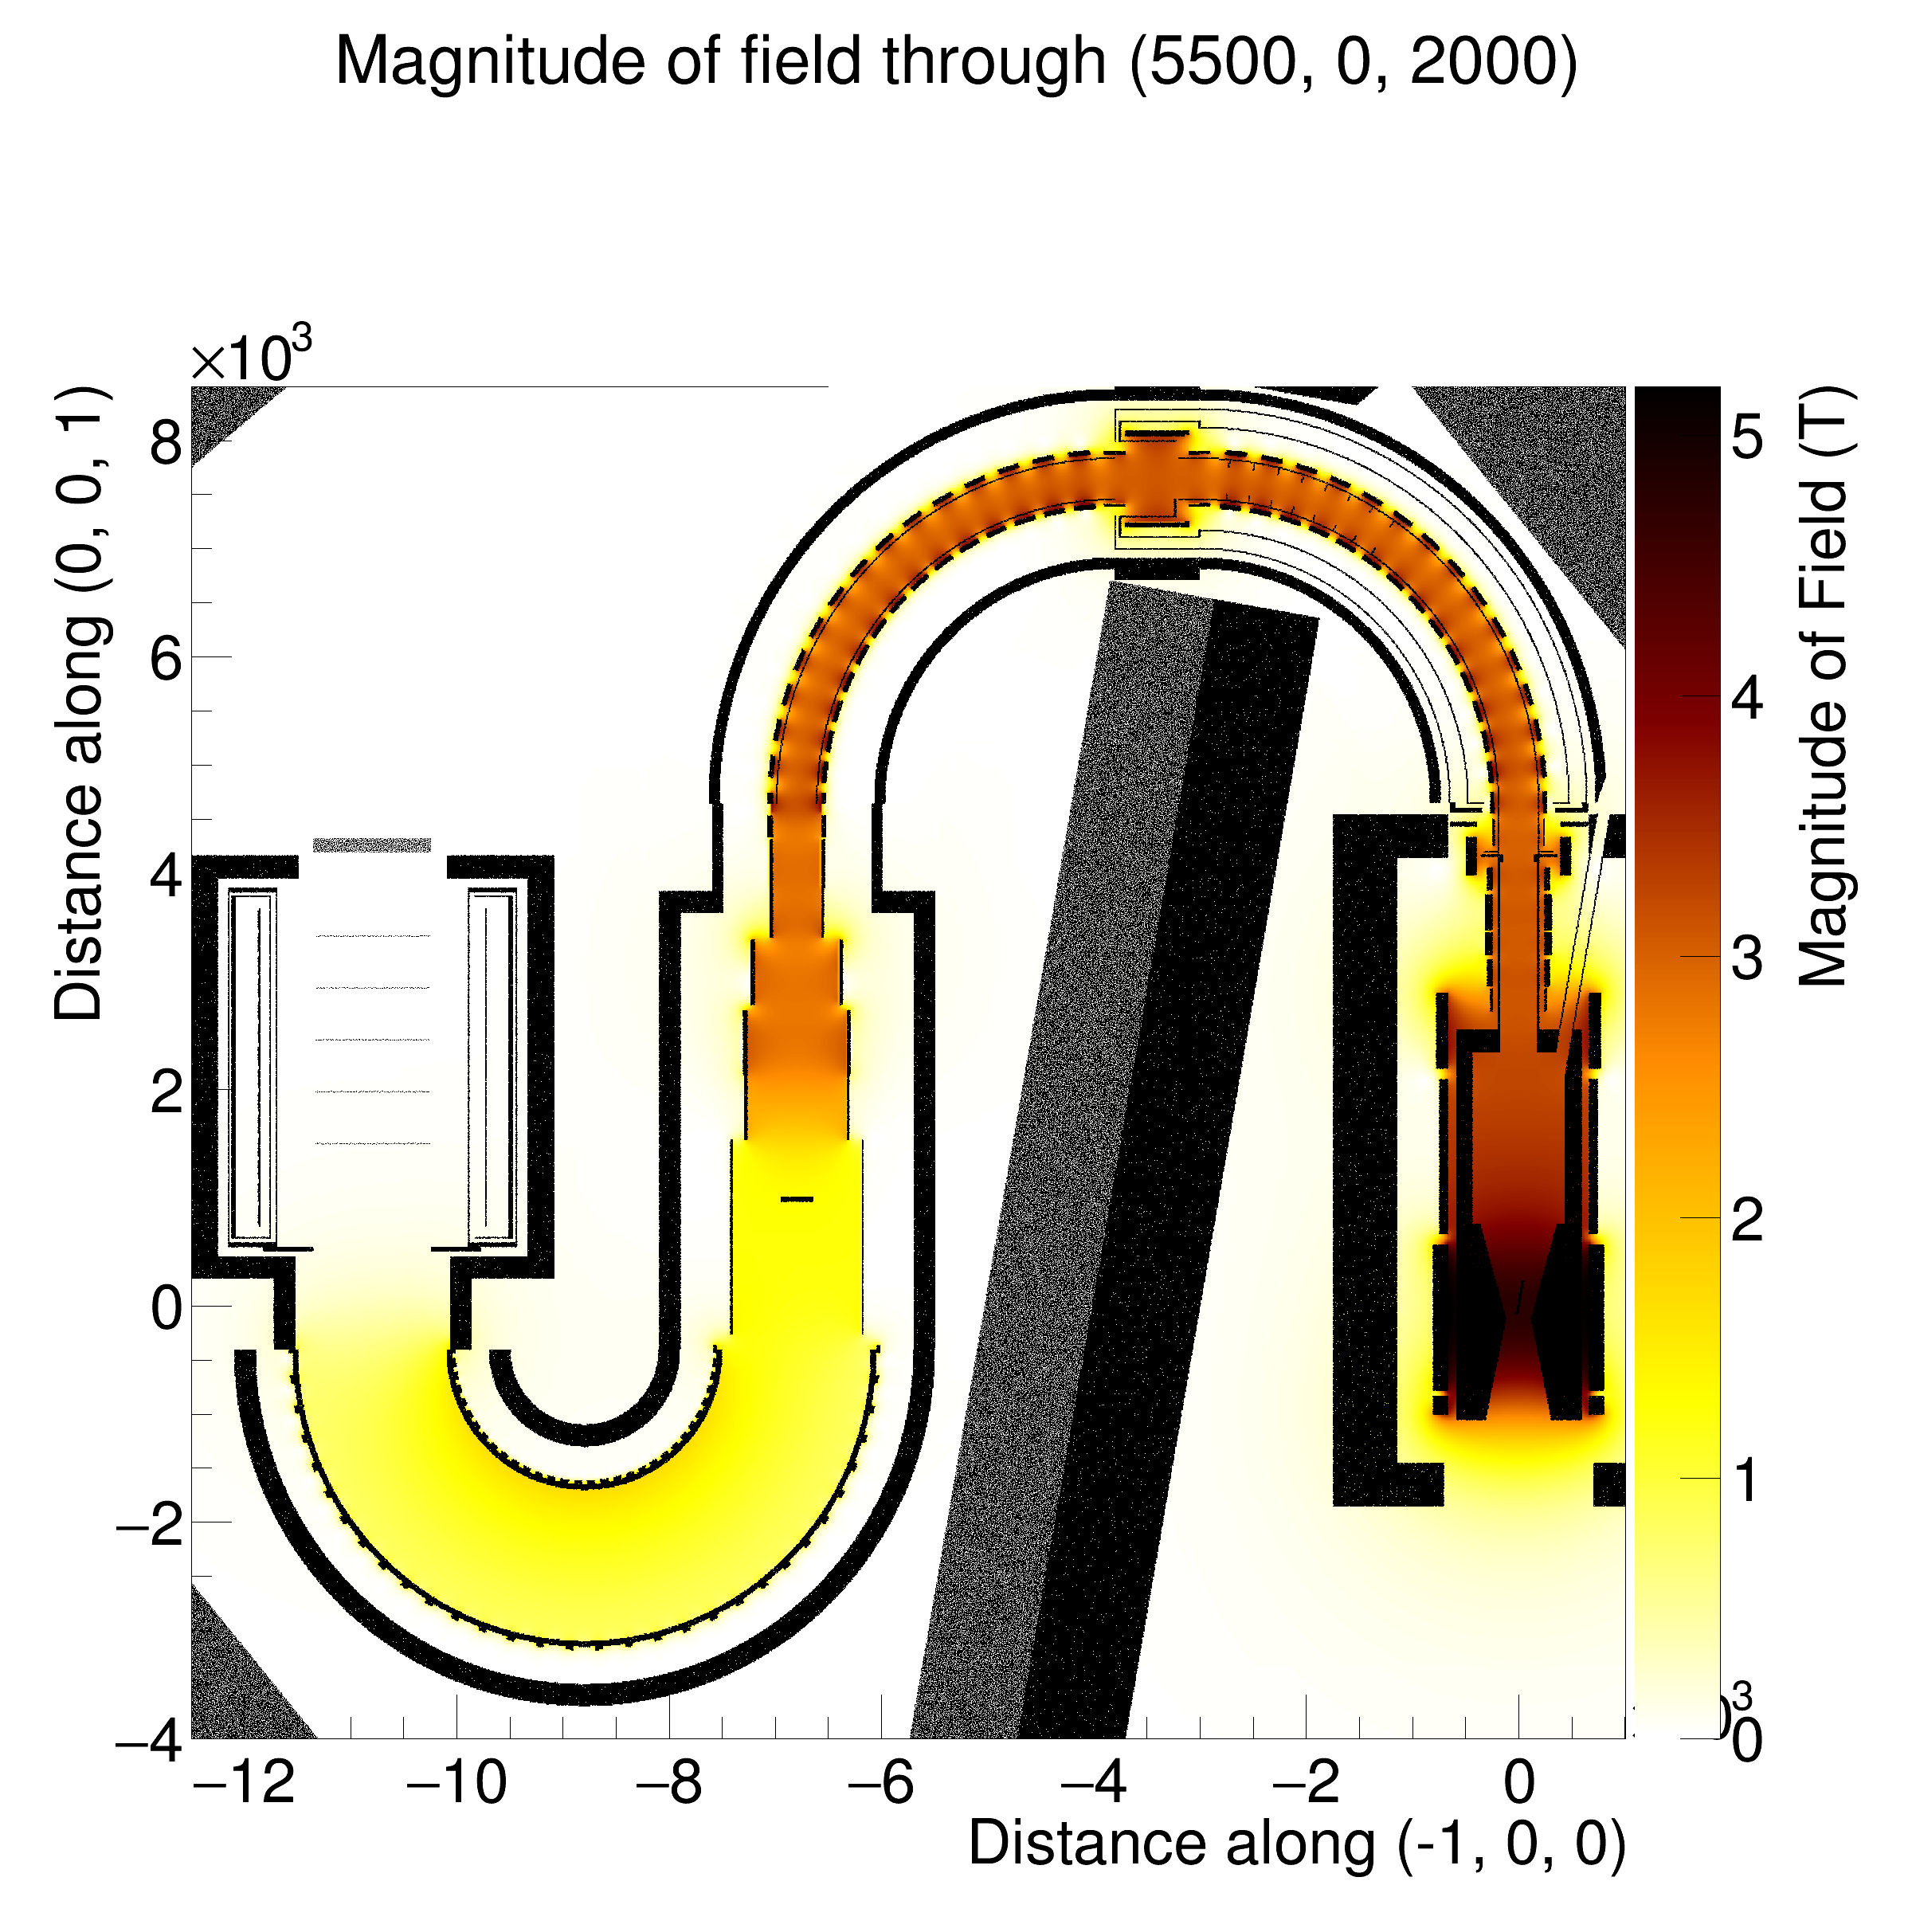
\includegraphics[width=0.45\textwidth,trim=0cm 0cm 0.0cm 13cm,clip=true]{figs/software/Plot_G4Beamline.png}
}
%}
\caption{
\figlabel{software:field}
Fieldmap produced by \protect\subref{fig:software:field:Opera} Opera and \protect\subref{fig:software:field:G4Beamline} G4Beamline.
Although the fringe field is larger with the G4Beamline calculation, the lack of material effects make this calculation less reliable.
Note that the G4Beamline calculation does not include the detector solenoid.
}
\end{figure}
}

\newcommand{\FigSoftwareFieldMapComparison}{
\begin{figure}[t]
\centering
%\fbox{
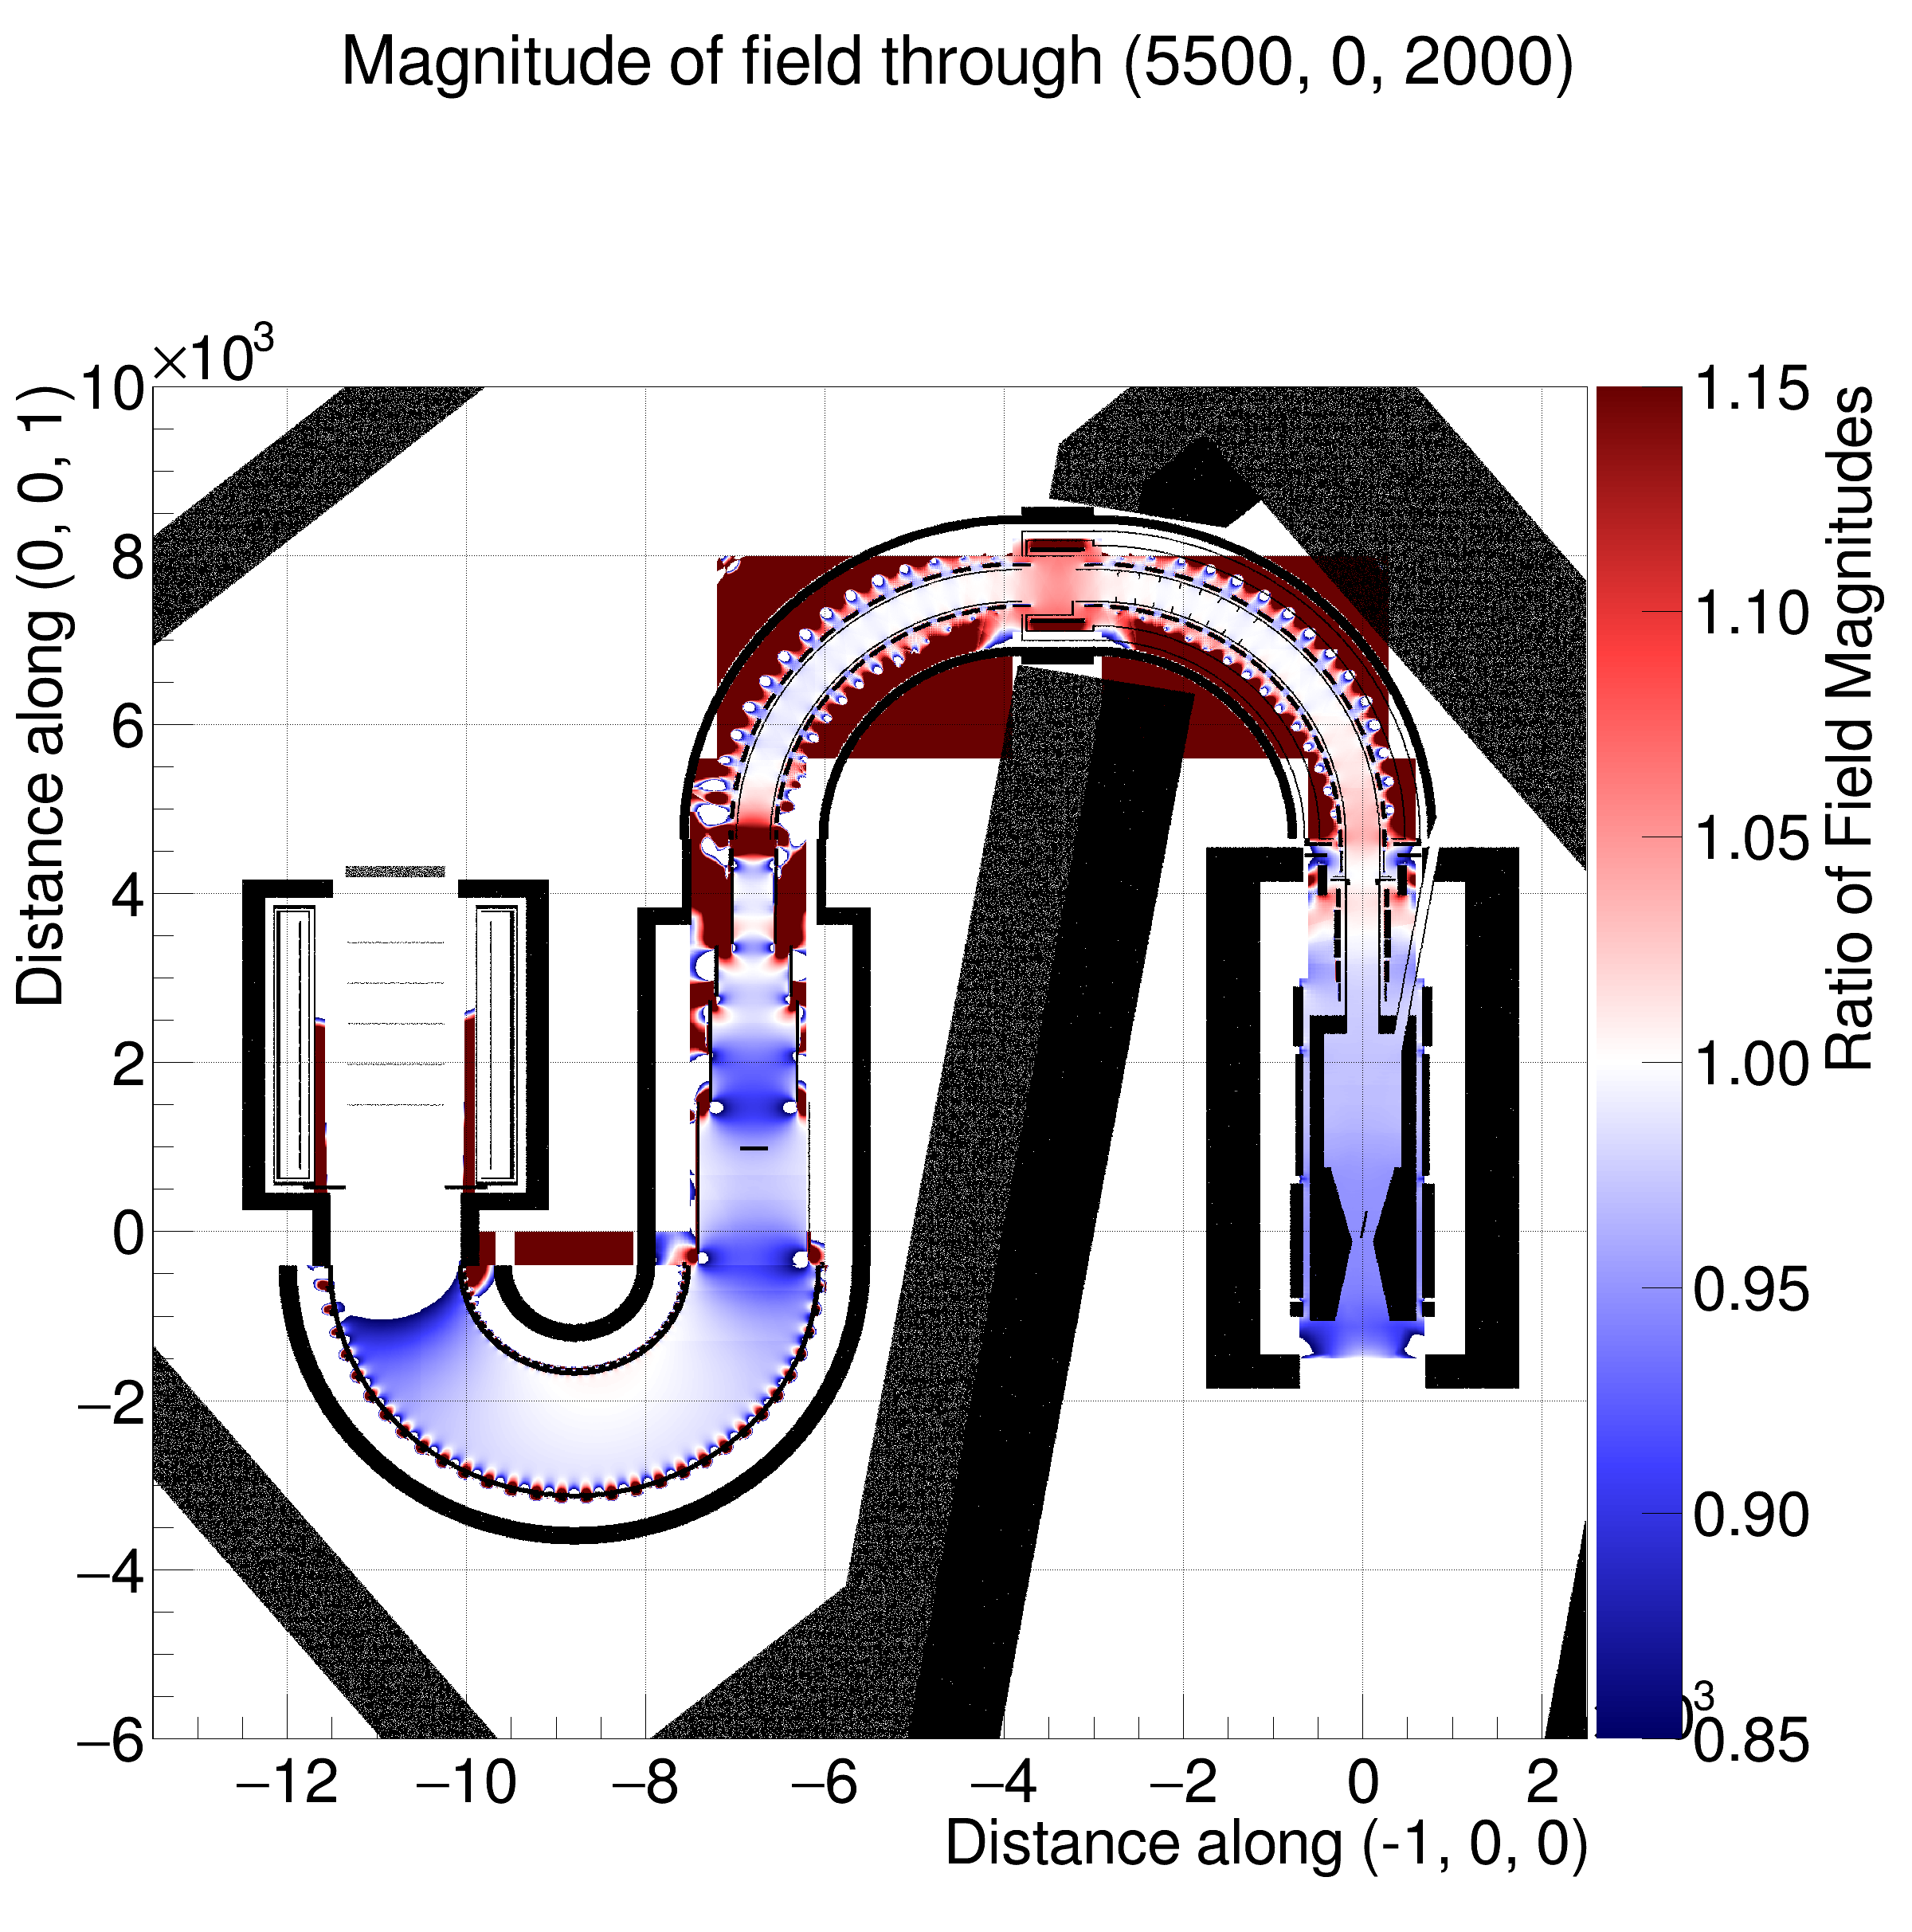
\includegraphics[width=0.9\textwidth,trim=0cm 0cm 0.0cm 13cm,clip=true]{figs/software/Plot_ratio_opera-G4Beamline.png}
%}
\caption{
\figlabel{software:field:comparison}
The ratio of the Opera and G4Beamline calculations shown in \fig{software:field}.
For most of the field within the beamline the calculations agree within 10\%, although around the ends of the solenoids the agreement is poorer.
}
\end{figure}
}

\newcommand{\FigSoftwareDipoleField}{
\begin{figure}[t]
\centering
%\fbox{
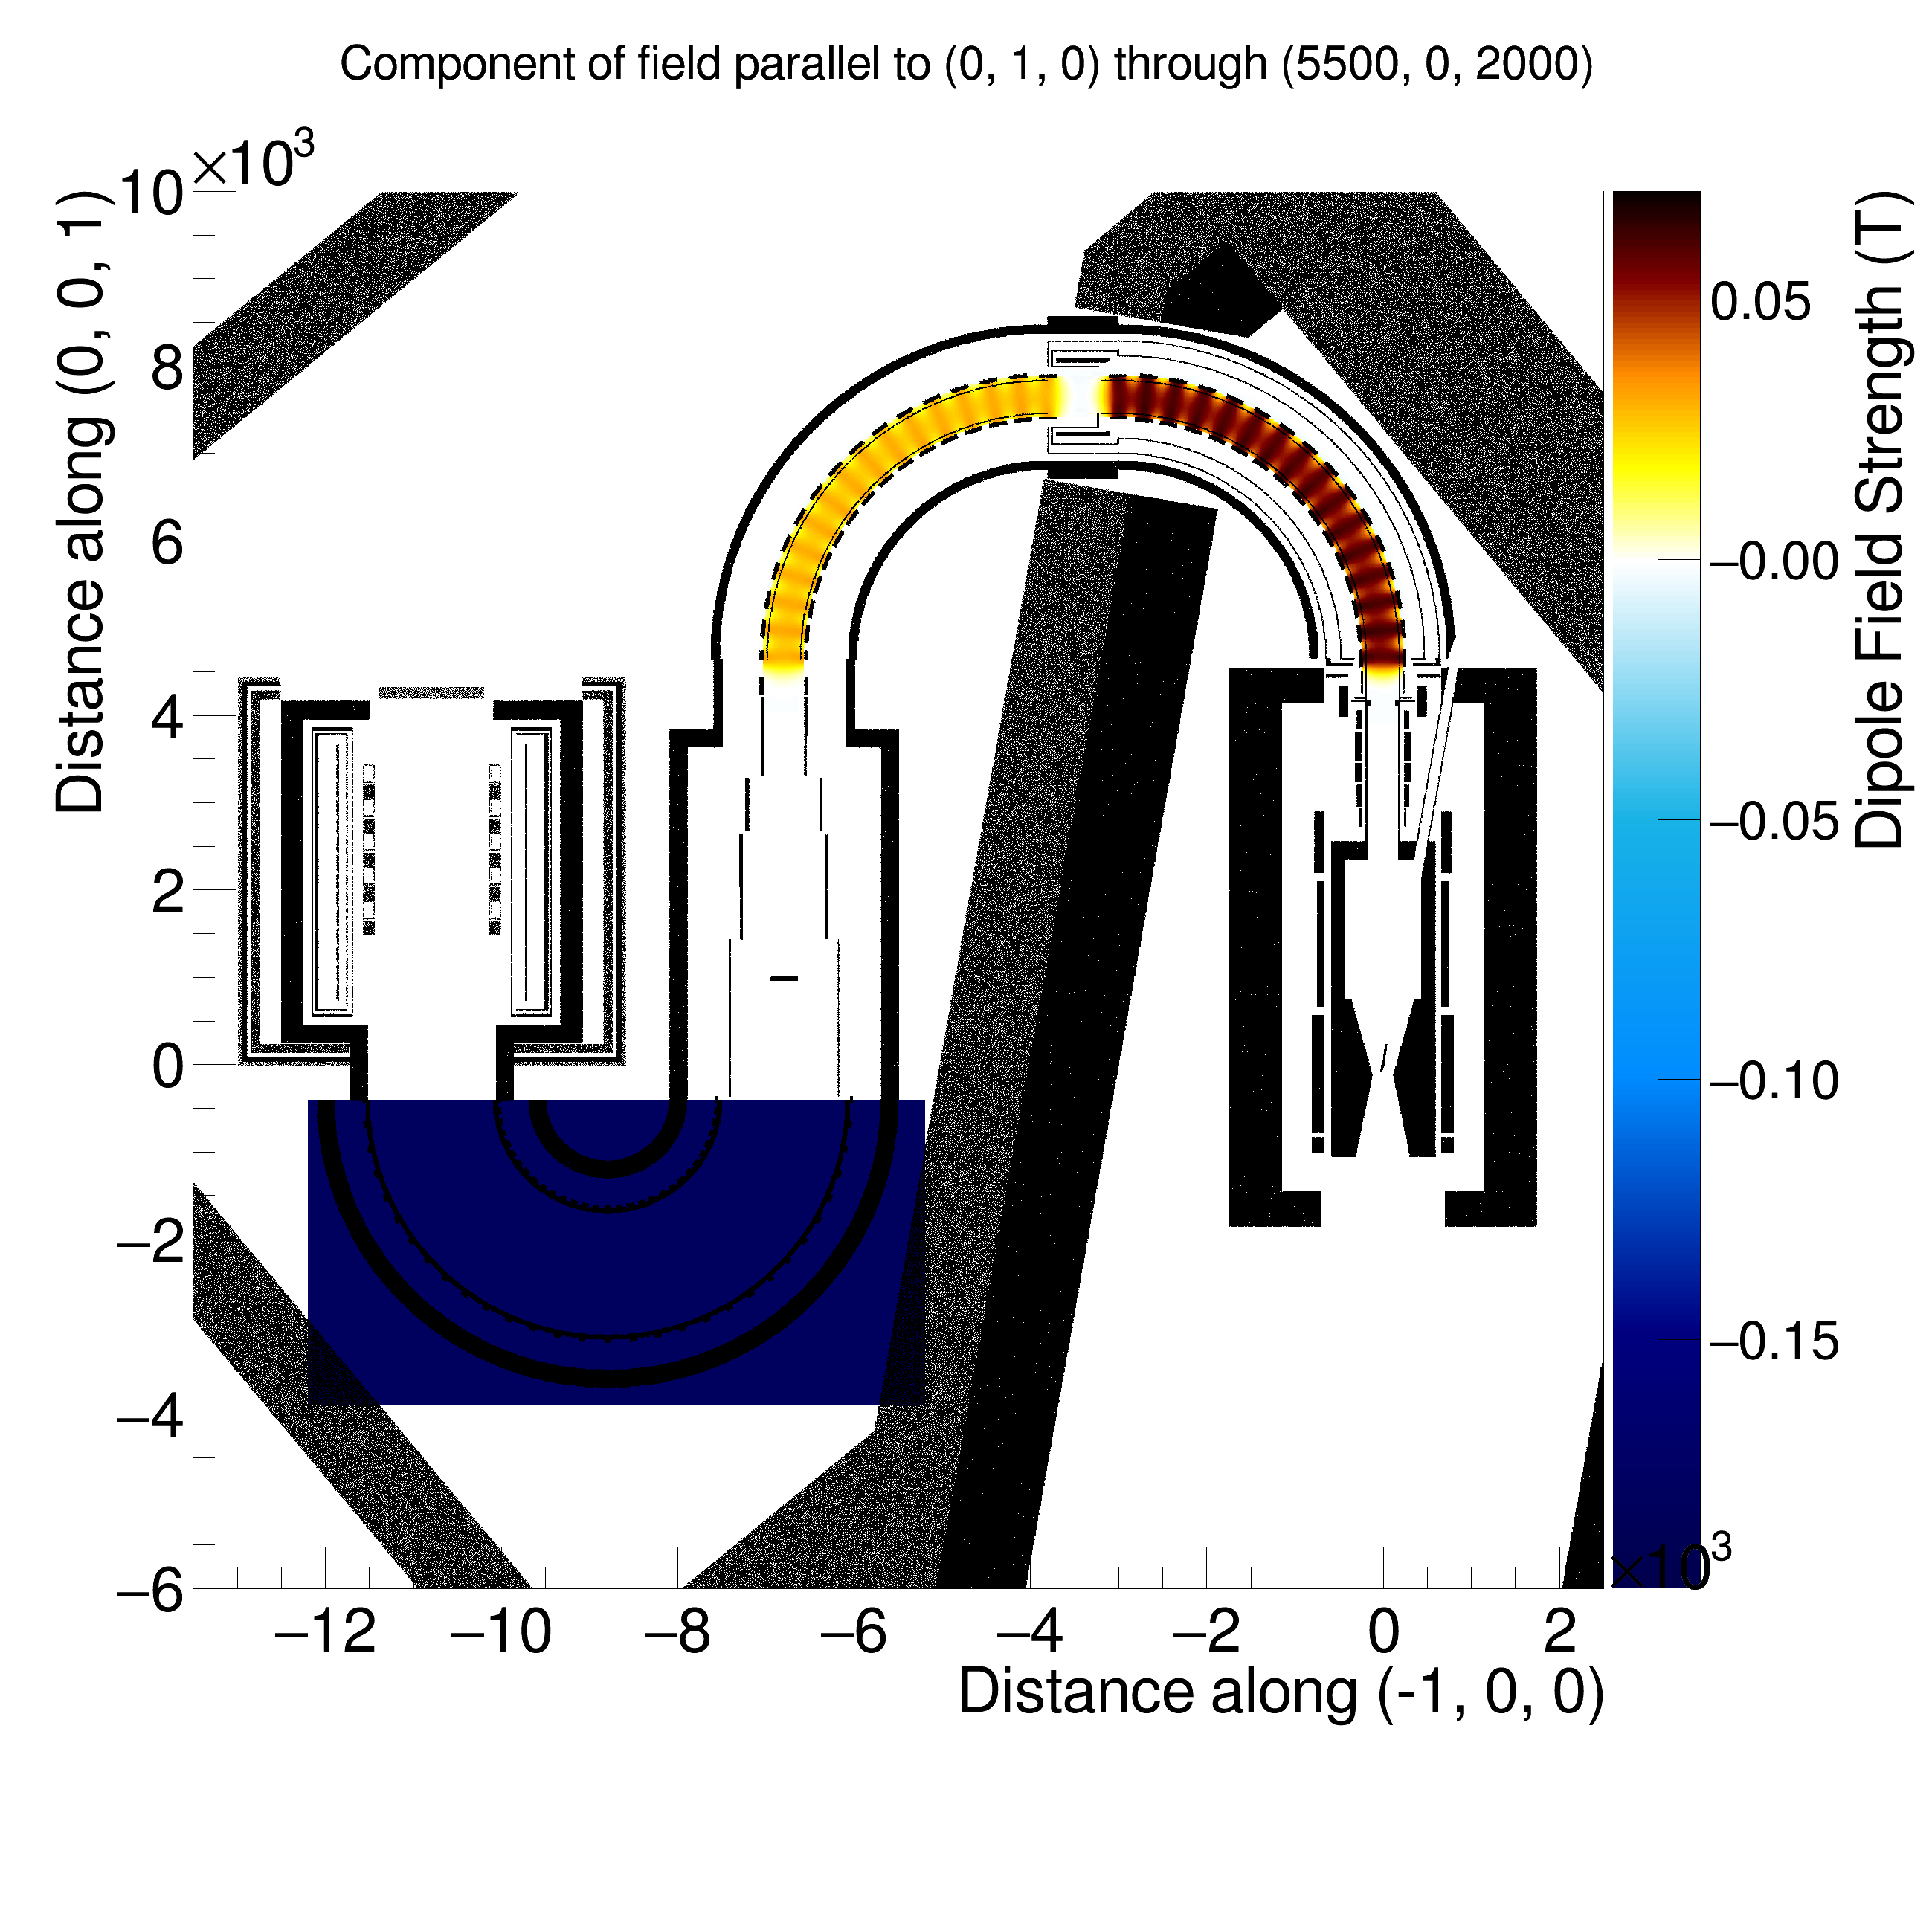
\includegraphics[width=0.9\textwidth,trim=2cm 8cm 0.0cm 6cm,clip=true]{figs/software/DipoleFields.png}
%}
\caption{
\figlabel{software:field:dipole}
The dipole field calculations used in ICEDUST for \phaseII. 
	The first 180\degree of the muon transport beamline have a positivie dipole field (pointing out of the plane)
	whilst the dipole along the electron spectrometer is negative and with a much larger strength.
	It can also be seen that the calculation for the dipole along the muon transport beamline contains realistic features (fringe fields, non-uniformities, etc)
	whilst the dipole field for the electron spectrometer is artificially uniform.  
}
\end{figure}
}

\chapter{Offline Software and The COMET Simulation}
In 2013 when I first worked on the COMET experiment, there were many disparate stand-alone simulations being run and no unified approach for data structures and analysis.
Since then, a single unified software framework has been prepared and is now being used throughout the collaboration.
Developing this framework has been a large part of my work over the last four years
, so this chapter presents both a summary of the framework and its development as well as an explanation of the techniques used.

\section{Developing the COMET Offline Framework}
Work to produce a common, standardised software framework for COMET began when funding was awarded for \phaseI.
With some four years to go before the switch on, it was clear that the support structure to handle and analyse the data needed to be in place soon.
Given the scale of the project and the available resources, the decision was taken to base the COMET offline framework on an existing one, which would reduce the amount of work needed and improve the reliability of the software since it would have been tested elsewhere.
A requirements document~\cite{COMETSoftwareRequirements} was drawn up with a list of items that the software should be able to do and a survey of existing experiments undertaken to build a list of candidate frameworks.
The list contained:
\begin{description}
\item [art] A framework being developed primarily at Fermilab~\cite{art:2011} which is also being used by Mu2e amongst other experiments.
\item [ND280] The framework~\cite{T2K:nim} used by the near detectors of the T2K experiment, which are also based at J-PARC.
\item [GAUDI] which is used by LHCb amongst other experiments~\cite{gaudi:2001}.
\item [MARLIN] The software being developed for the International Linear Collider (ILC)~\cite{marlin:web}.
\end{description}

The final decision was to use the ND280 framework\footnote{The term `ND280' can
refer to one of either the ND280 detector itself, the site at J-PARC that
houses both the ND280 and INGRID detectors, or the software used to analyse and
simulate the T2K near-detectors.  For the purposes of this chapter, unless
specified explicitly, the term `ND280' should be taken as referring to the
software.} 
since GAUDI and MARLIN would have required to much effort to adapt to the COMET
requirements; since art is used by Mu2e and keeping the software distinct is
important for the two experiments to co-exist as cross-checks; and because the
ND280 software was already known to a large part of the COMET collaboration and
had been tested on real data at J-PARC.

\FigNDTwoEighty
\Fig{software:ND280} shows an overview of the ND280 framework, including its package structure and the various interactions between packages.

With the decision to base the COMET experiment on the ND280 framework -- and with the selection of the new name: `ICEDUST' -- the process of forking the software was begun.
Since the ND280 framework had evolved somewhat organically a review of the conventions and code names was performed.
For example, whilst the ND280 software prefixes all classes with a capital `T', the ICEDUST conventions~\cite{ID:conventions} agreed to swap this to a capital `I' to reduce clashes with ROOT which also uses `T'.
The package renaming scheme~\cite{ID:packageRenaming} was developed so that the purpose of a package and its role with the other packages could be more clearly identified.

Whilst fundamental, low-level packages have been left relatively unchanged higher-level packages which include more detector specific details had to be developed.
Additionally some aspects of COMET needed considerably more support than had been present in the ND280 software.
Some of the key changes that have been introduced between ICEDUST and ND280 are:
\begin{description}
	\item [Simulation] Although the fundamental data types have not been changed, the simulation has been nearly completely rewritten.
		In particular, support for hadron production codes have been added to model the production target;
		both the Geant4-based package (renamed to SimG4) and the detector response simulation (renamed as SimDetectorResponse) were given near-total makeovers;
		a new package (SimHitMerger) for resampling the G4Hits (simulated charge or energy deposits) was added.
		Custom physics models have been added to SimG4 to improve the modelling of the COMET-specific physics processes.
	\item [Magnetic Field handling]  whilst the ND280 detector has a fairly straight-forward magnetic field, the COMET experiment has anything but this.  
		Accordingly significant work has been made to replace the way
		the magnetic field was handled from essentially a few constants
		to the ability to use complete fieldmap descriptions made with
		external field calculation software.
	\item [Geometry handling] The unusual shape of the COMET experiment, the level of detail needed for background estimations in a high-precision experiment, and the changing nature of a staged experiment meant a more elaborate scheme for handling the geometry was necessary than had existed in ND280.
	\item [Reconstruction and Calibration packages] As simply renaming of the packages, the interdependence of the calibration and reconstruction packages has been improved.
		Additionally, support for track fitting using Genfit2~\cite{genfit-Hoppner:2009af} has been added as well as new track finding algorithms being developed.
\end{description}

In addition to the above changes to the way the software runs, the distribution of the software has changed from using CMT~\cite{cmt} with CVS version control to being based on git with a GitLab~\cite{GitLab} web-based user interface for the official repository.
The switch to GitLab also brought a `merge-request' which has allowed development of ICEDUST to progress rapidly with only a small number of developers.
Although initially the intention was also to switch the build system from CMT to CMake~\cite{cmake}, this decision has since been reversed due to improvements in CMT.

In the 3 years since the initial work forking ND280 to produce ICEDUST in summer 2013 some 3,200 commits have edited about two million lines of code in the official version of the framework.
This has been the work of some 25 collaborators whilst about 15 other users have GitLab accounts and use the software.
ICEDUST has been used to run three large Monte Carlo productions, most recently simulating about $10^{11}$~\ac{POT} events -- equivalent to 18,000 \phaseI bunches -- in some 100~TB of simulated data.

\section{Overview of ICEDUST}
ICEDUST Can Efficiently Do Useful Software Things and stands for the Integrated COMET Experiment Data User Software Toolkit.
\Fig{software:ICEDUSTOverview} shows the flow of data through the different packages of the framework and the data formats used.

\FigICEDUSTOverview

Inside the framework, nearly all processing is done using a ROOT file-based format known as oaEvent.  
Files of this type contain header information providing run identification numbers as well as a description of the geometry and magnetic field.  
The data payload contained in oaEvent files is stored in a ROOT TTree with a single branch containing a single COMET event per entry.
Each COMET event has a dynamic structure and can have any object which derives from the IDatum base class added to its list of data on an event-by-event basis.

Data from the detector systems is recorded in MIDAS~\cite{MIDAS} format which also contains data from the slow control monitors such as temperature sensors and high-voltage power supplies.
The task of converting the MIDAS files into the oaEvent format is handled by the package oaUnpack which writes out new, converted files, and oaRawEvent which can convert the MIDAS files to oaEvent format on the fly.

Simulated data is also produced in the oaEvent format and involves some 4 to 6 packages being called, described in more depth in section~\sect{COMETSim}.

Once either simulated data has been produced or real data has been converted, calibration routines can then be applied.
Each sub-detector is capable of pulling constants that were previously generated from a MySQL database and applying these to the detected (or simulated) energy deposits.
These calibrated hits are then passed into the reconstruction stage.  
Here again each sub-detector system is first allowed to handle the data until a full reconstructed event is produced.
For the tracking detectors this stage typically involves an initial track finding stage, where noise hits are removed and track candidates consisting of a list of hits are collected, and secondly a track fitting stage where the actual path of the underlying particle is reconstructed and key values like momentum and helical pitch-angle deduced.

Nearly all of the processing of data up to this stage has used the oaEvent format.
The final analysis stage however moves into a simpler, flatter format, known as oaAnalysis, which produces a data summary tree (as opposed to tape) that can be accessed without a dependence on the full ICEDUST software.

Around all of this there are several utility packages, such as the event display which can visualise any oaEvent file, and IcedustControl which can run a single set of data through the data chain and is the main steering mechanism used for production running.

\section{The COMET Simulation}
\sectlabel{COMETSim}
\FigSimulationOverview
The ability for an experiment to set stringent confidence limits in the event of a null-observation is determined both by the expected signal acceptance (which should be high) and the predicted number of background events (which should be low).
For COMET's target single-event sensitivity -- which is only a measure of the signal efficiency -- to translate to a comparable confidence limit if no signal is observed, fewer than one background events should occur during the run.
By comparison, some $10^{18}$ and $10^{21}$~protons \CHECK{Is this the right number of protons on target?} will impinge the production target in \phaseI and \phaseII respectively so it is clear that the ability to suppress backgrounds must be demonstrably high.

Simulation plays a crucial role in making such a demonstration. 
Before the experiment is built and operated it allows one to optimise crucial aspects of the geometry and parameters, such as the magnetic field strengths or timing cuts.
In addition, using Monte Carlo techniques in an accurate simulation allows an estimation of the background rate by sampling the parameter space corresponding to each stage of the experiment.
Clearly then the simulation itself must be as faithful a reproduction of the true experiment as possible.


The COMET simulation therefore needs to be both highly accurate and highly efficient.
As well as custom physics modelling, and special handling for the magnetic field, several resampling techniques have been introduced to increase the statistical power.
The steps needed to build up the COMET simulation are shown in \fig{software:SimulationOverview}.

To reduce the uncertainties associated with the production target and the muon and pion yield multiple hadron codes can be used, including PHITS~\cite{PHITS2002}, MARS~\cite{MARS1995}, Fluka~\cite{FLUKA2005} and Geant4~\cite{Geant42003}.
The SimG4 package, which is based on Geant4, then takes over the muon beam simulation and tracking of particles to the detectors.
These energy deposits, referred to as G4Hits, can then be converted to realistic electronic detector-readouts by the SimDetectorResponse package.
Often though, the G4Hits are first reshuffled with G4Hits from other events.  
Since one event coming out from SimG4 is 

\subsection{Handling Geometry}

\subsection{Field Calculation}

\subsection{Production Target Simulations}

\subsection{Extending the Geant4 Physics Modelling}

\subsection{Resampling With the Hit Merger}
